\documentclass[preprint,10pt]{elsarticle}
\pdfoutput=1
\usepackage{graphicx}
\usepackage{caption}
\usepackage[labelformat=simple]{subcaption}
\renewcommand{\thesubfigure}{(\roman{subfigure})}
\usepackage{amsmath}
\usepackage{amssymb}
\usepackage{amsthm}
\usepackage{setspace}
 \usepackage[normalem]{ulem} % strike through
\usepackage{cancel}
\usepackage[linesnumbered,ruled,vlined,noend]{algorithm2e}
\usepackage{algpseudocode}% http://ctan.org/pkg/algorithmicx
% \usepackage{tabularray} %for new style table
% \UseTblrLibrary{booktabs}
% \usepackage{amsthm}
\usepackage{color}
\usepackage[]{color}
\usepackage[]{url}
\usepackage{hyperref}
\usepackage{cleveref}
\usepackage{enumerate}
\usepackage{enumitem}

 
 
\usepackage{tikz}
\usepackage{standalone}
\usetikzlibrary{arrows}
\usetikzlibrary{decorations} 
\usetikzlibrary{decorations.markings}
\usetikzlibrary{decorations,fit,shapes} 
\usetikzlibrary{arrows.meta,positioning}
\usetikzlibrary{shapes.misc}


\newcommand{\HR}{\mbox{{\sf HR}}}
\newcommand{\HRTLQ}{\mbox{{\sf HR2LQ}}}
\newcommand{\SCTLQ}{\mbox{{\sf SC2LQ}}}
\newcommand{\prefa}{\mbox{{\sf Pref($a$)}}}
\newcommand{\preflqa}{\mbox{{\sf PrefLQ($a$)}}}
\newcommand{\prefb}{\mbox{{\sf Pref($b$)}}}
\newcommand{\prefh}{\mbox{{\sf Pref($h$)}}}
\newcommand{\preflqh}{\mbox{{\sf PrefLQ($h$)}}}
\newcommand{\prefr}{\mbox{{\sf Pref($r$)}}}
\newcommand{\prefsh}{\mbox{{\sf PrefS($h$)}}}
\newcommand{\prefslqh}{\mbox{{\sf PrefSLQ($h$)}}}
\newcommand{\prefsa}{\mbox{{\sf PrefS($a$)}}}
\newcommand{\prefsaa}{\mbox{{\sf PrefS($a'$)}}}
\newcommand{\prefslqa}{\mbox{{\sf PrefSLQ($a$)}}}
\newcommand{\prefu}{\mbox{{\sf Pref($u$)}}}
\newcommand{\prefv}{\mbox{{\sf Pref($v$)}}}
\newcommand{\prefal}{\mbox{{\sf List($a$)}}}
\newcommand{\SCLQ}{\mbox{{\sf SCLQ}}}
\newcommand{\HRLQ}{\mbox{{\sf HRLQ}}}
\newcommand{\HRLQT}{\mbox{{\sf HR-1TLQ}}}
\newcommand{\RSM}{\mbox{{\sf RSM}}}
\newcommand{\CRSM}{\mbox{{\sf CRITICAL-RSM}}}
\newcommand{\POP}{\mbox{{\textsc{AlgoPop}}}}
\newcommand{\MMLQ}{\mbox{{\sf MM2LQ}}}
\newcommand{\MMTLQ}{\mbox{{\sf MM-1T-2LQ}}}
\newcommand{\MMTTLQ}{\mbox{{\sf MM-2T-2LQ}}}
\newcommand{\SMTTLQ}{\mbox{{\sf SM-2T-2LQ}}}
\newcommand{\HRTTLQ}{\mbox{{\sf HR-2T-2LQ}}}
\newcommand{\LQ}{\mbox{{\sf LQ}}}
\newcommand{\HRLQCL}{\mbox{{\sf HRLQCL}}}

\newcommand{\CL}{\mbox{{\sf CL}}}
\newcommand{\Df}[1]{\mbox{{\sf $def(#1)$}}}
\newcommand{\Dfa}[1]{\mbox{{\sf $def_{\mathcal{A}}(#1)$}}}
\newcommand{\Dfb}[1]{\mbox{{\sf $def_{\mathcal{B}}(#1)$}}}
\newcommand{\Dfh}[1]{\mbox{{\sf $def_{\mathcal{H}}(#1)$}}}
\newcommand{\Dfr}[1]{\mbox{{\sf $def_{\mathcal{R}}(#1)$}}}
\newcommand{\MAXEFM}{\mbox{{\sf MAXEFM}}}
\newcommand{\MAXSMTI}{\mbox{{\sf MAX SMTI}}}
\newcommand{\CLIQUE}{\mbox{{\sf CLIQUE}}}
\newcommand{\minBP}{\mbox{{\sf MinBP}}}
\newcommand{\minBR}{\mbox{{\sf MinBR}}}
\newcommand{\ESDA}{\mbox{{\sf ESDA}}}
\newcommand{\MSDA}{\mbox{{\sf MSDA}}}
\newcommand{\CSM}{\mbox{{\sf CSM}}}
\newcommand{\HRTMSLQ}{{\sf{HRT}\text{-}\sf{MSLQ}}}
\newcommand{\HH}{\mathcal{H}}
\newcommand{\RR}{\mathcal{R}}
\renewcommand{\AA}{\mathcal{A}}
\newcommand{\BB}{\mathcal{B}}
\newcommand{\RRLQ}{\mathcal{R}_{lq}}
\newcommand{\HHLQ}{\mathcal{H}_{lq}}
\newcommand{\AALQ}{\mathcal{A}_{lq}}
\newcommand{\AANLQ}{\mathcal{A}_{nlq}}
\newcommand{\BBLQ}{\mathcal{B}_{lq}}
\newcommand{\BBNLQ}{\mathcal{B}_{nlq}}
\newcommand{\CSMTIML}{\mbox{{\sf COMPLETE SMTI-2ML}}}
\newcommand{\lst}{list}
\newcommand{\lqlst}{lqlist}
\newcommand{\clst}{clonedlist}
\newcommand{\D}{\mathcal{D}}
\newcommand{\EE}{\mathcal{E}}
\newcommand{\clr}{\textcolor{blue}}
\newcommand{\clrG}{\textcolor{gray}}
\newcommand{\clrP}{\textcolor{purple}}
\newcommand{\rvrTh}{\textcolor{cyan}}
\newcommand{\clrR}{\textcolor{red}}
% \newcommand{\comment}{\textcolor{red}}
\renewcommand{\S}{{s}}
\newcommand{\T}{{t}}


\newtheorem{property}{Property}
\newtheorem{cl}{Claim}
\newtheorem{definition}{Definition}
\newtheorem{theorem}{Theorem}
\newtheorem{lemma}[theorem]{Lemma}
\newtheorem{observation}{Observation}
\newtheorem{remark}{Remark}


\definecolor{lightgray}{rgb}{0.83, 0.83, 0.82}

\tikzset{cross/.style={cross out, draw=black, minimum size=2*(#1-\pgflinewidth), inner sep=0pt, outer sep=0pt},
	%default radius will be 1pt. 
	cross/.default={1pt}}
\usetikzlibrary{arrows, decorations.pathmorphing}

\tikzstyle{vertex}=[auto=left,circle,draw=black!80,fill=none,minimum size=15pt,inner sep=0pt]

%tik picture
%\usepackage{comment}
\tikzset{
    photon/.style={decorate, decoration={snake}, draw=red}} 

\newcommand\blfootnote[1]{%  footnote without marker
  \begingroup
  \renewcommand\thefootnote{}\footnote{#1}%
  \addtocounter{footnote}{-1}%
  \endgroup
}


    

% \newenvironment{appendix-lemma}[1]{\vspace{\theorempreskipamount}\noindent{\bf Lemma~#1~} \em }{\vspace{\theorempostskipamount}}
\newcommand{\etal}{\textit{et al}.}


\newenvironment{appendix-lemma}[1]{\vspace{0.1in}\noindent{\bf Lemma~#1~} \em }{\vspace{0.1in}}
\newenvironment{appendix-claim}[1]{\vspace{0.1in}\noindent{\bf Claim~#1~} \em }{\vspace{0.1in}}
\newenvironment{appendix-theo}[1]{\vspace{0.1in}\noindent{\bf Theorem~#1~} \em }{\vspace{0.1in}}
\newenvironment{appendix-prop}[1]{\vspace{0.1in}\noindent{\bf Property~#1~} \em }{\vspace{0.1in}}


\newenvironment{proced}[1][htb]{%
    \renewcommand{\algorithmcfname}{Procedure}% Update algorithm name
    \begin{algorithm}[#1]%
    \renewcommand{\thealgocf}{}% Remove procedure number
}{%
    \end{algorithm}%
}


\algrenewcommand{\algorithmiccomment}[1]{\hfill\hfill\hfill\hfill\hfill\hfill\hfill// #1}

\renewenvironment{proof}{{\textit{Proof:}}}{\qed}
\newcommand{\proofofref}{}
\newproof{zproofof}{Proof of \proofofref}
\newenvironment{proofof}[1] {\renewcommand{\proofofref}{#1}\zproofof}
 {\endzproofof}

% \usepackage{lineno}
 % \linenumbers

 
\usepackage[margin = 1.2in]{geometry}

%TODO Please add
\title{Critical Relaxed Stable Matchings with Ties in the Many-to-Many Setting\tnoteref{label1}}
\tnotetext[]{A preliminary version~\cite{nasre2023critical} of this work appeared in 49th International Workshop on Graph-Theoretic Concepts in Computer Science 2023 (WG 2023)} 

%% The lineno packages adds line numbers. Start line numbering with
%% \begin{linenumbers}, end it with \end{linenumbers}. Or switch it on
%% for the whole article with \linenumbers.
% \usepackage{lineno}
\journal{SIAM Journal on Discrete Mathematics}
\begin{document}

\begin{frontmatter}


%% Title, authors and addresses

%% use the tnoteref command within \title for footnotes;
%% use the tnotetext command for theassociated footnote;
%% use the fnref command within \author or \address for footnotes;
%% use the fntext command for the associated footnote;
%% use the corref command within \author for corresponding author footnotes;
%% use the cortext command for theassociated footnote;
%% use the ead command for the email address,
%% and the form \ead[url] for the home page:

\author[1]{Meghana Nasre}
\ead{meghana@cse.iitm.ac.in}
% \ead[url]{http://www.cse.iitm.ac.in/~meghana}
\affiliation[1]{organization={Department of CSE},
            addressline={IIT Madras},
            city={Chennai},
            postcode={600036}, 
            state={Tamilnadu},
            country={India}}
    % \fntext[fn1]{Partially funded by SERB grant CRG/2019/004757.}
            
\author[2]{Prajakta Nimbhorkar}
\ead{prajakta.nimbhorkar@gmail.com}
% \ead[url]{http://www.cmi.ac.in/~prajakta/}

\affiliation[2]{organization={Department of CSE},
            addressline={Chennai Mathematical Institute and UMI ReLaX},
            city={Chennai},
             postcode={603103}, 
            state={Tamilnadu},
            country={India}}
    % \fntext[fn2]{Partially funded by Infosys Grant and SERB grant CRG/2019/004757.}

            
\author[1]{Keshav Ranjan}  
\ead{ranjankeshav08@gmail.com}

%% use optional labels to link authors explicitly to addresses:



% \listoftodos

%TODO mandatory: add short abstract of the document
\begin{abstract}
We study the many-to-many bipartite matching problem in the presence of preferences where ties, as well as lower quotas, may appear on both sides of the bipartition. The input is a bipartite graph $G=(\AA \cup \BB, E)$, where each vertex in $\AA \cup \BB$ has a positive upper quota and a non-negative lower quota denoting the maximum and minimum number of vertices that can be assigned to it from its neighborhood. Additionally, each vertex specifies a preference ordering, possibly containing ties, over its neighbors. 
A \emph{critical} matching is a matching which fulfills vertex lower quotas to the maximum possible extent. We seek to compute a matching that is critical as well as optimal with respect to the preferences of vertices.  Stability, a well-accepted notion of optimality in the presence of two-sided preferences, is generalized to weak-stability in the presence of ties. However, a matching that is critical as well as weakly stable may not exist. Popularity is another well-investigated notion of optimality for the two-sided preference model; however, in the presence of ties (even without lower quotas), a popular matching may not exist. We, therefore, consider the notion of relaxed stability, which was introduced and studied by  Krishnaa, Limaye, Nasre, and Nimbhorkar~(JoCO 2023). We show that a critical matching that is relaxed stable always exists, although computing a maximum-size relaxed stable matching turns out to be NP-hard. 
Our main contribution is a $\frac{3}{2}$-approximation algorithm for computing a maximum-size critical relaxed stable matching. 
\end{abstract}

\begin{keyword}
Stable Matching \sep Relaxed Stable Matching \sep Ties in Preferences \sep Approximation Algorithms


%% or \MSC[2008] code \sep code (2000 is the default)
 \MSC[2020] 05C85 \sep 68W25 
 % \textit{MSCcodes:} 05C85 \clr{Graph algorithms}, 68W25 \clr{Approximation algorithms}

\end{keyword}


\end{frontmatter}


\section{Introduction}
\label{sec:introduction}

Suppose that we want to \emph{fit} and \emph{validate} a model on the basis of a single dataset.  Two example scenarios are as follows:
\begin{list}{}{}
\item{\emph{Scenario 1.}} We  want to use the data both to generate and to test a hypothesis. 
\item{\emph{Scenario 2.}} We want to use the  data both to fit a complicated model, and to obtain an accurate estimate of the expected prediction error. 
\end{list}
In either case, it is clear that a naive approach that fits and validates a model on the same data is deeply problematic. In Scenario 1, testing a hypothesis on the same data used to generate it will lead to hypothesis tests that do not control the Type 1 error, and to confidence intervals that do not attain the nominal coverage \citep{fithian2014optimal}.   And in Scenario 2, estimating the expected prediction error on the same data used to fit the model will lead to massive downward bias  \citep[see][for recent reviews]{tian2020prediction,oliveira2021unbiased}.

In the case of Scenario 1, recent interest  has focused on \emph{selective inference}, a framework that enables a data analyst to generate and test a hypothesis on the same data \citep[see, e.g.,][]{taylor2015statistical}. The main idea is as follows: to test a hypothesis generated from the data, we should condition on the event that we selected this particular hypothesis. Despite promising applications of this framework to a number of problems, such as inference after regression \citep{lee2016exact}, changepoint detection \citep{jewell2022testing,hyun2021post}, clustering \citep{gao2020selective,chen2022selective,yun2023selective}, and outlier detection \citep{chen2020valid}, it suffers from some drawbacks: 
\begin{enumerate}
\item To perform selective inference, the  procedure used to generate the null hypothesis must be fully-specified in advance.  For instance, if a researcher wishes to cluster the data and then test for a difference in means between the clusters, as in \cite{gao2020selective} and \cite{chen2022selective}, then they must fully specify the clustering procedure (e.g., hierarchical clustering with squared Euclidean distance and complete linkage, cut to obtain $K$ clusters) in advance. 
\item Finite-sample selective inference typically requires an assumption of multivariate Gaussianity, though in some cases this can be relaxed to obtain asymptotic results \citep{taylor2018post,tian2017asymptotics,tibshirani2018uniform,tian2018selective}.
\end{enumerate}
Thus, it is clear that selective inference does not provide a flexible, ``one-size-fits-all" approach to Scenario 1. 

In the case of Scenario 2, proposals to de-bias the ``in-sample" estimate of expected prediction error  tend to be specialized to simple models, and thus do not provide an all-purpose tool that is broadly applicable to complex contemporary settings \citep{oliveira2021unbiased}.

\emph{Sample splitting} \citep{cox1975note} is an intuitive  approach that is broadly applicable to a variety of settings, including Scenarios 1 and 2; see the left-hand panel of Figure~\ref{fig:samplesplit_vs_datathin}. We split a dataset containing $n$ observations into two sets, containing $n_1$ and $n_2$ observations, respectively (where $n_1+n_2=n$). Then we can generate a hypothesis based on the first set and test it on the second set (Scenario 1), or we can fit a model to the first set and estimate its error on the second set (Scenario 2). Sample splitting also forms the basis for cross-validation, an important tool for a practicing data scientist \citep{hastie2009elements}. 

While sample splitting often can 
 adequately address both Scenarios 1 and 2, it also suffers from some drawbacks: 
\begin{enumerate} 
    \item If the data contain outliers, then each outlier is assigned to a single subsample. %Again, this may not be desirable.
    \item If the observations are not independent (for instance, if they correspond to a time series) then the subsamples that result from sample splitting are not independent, and so sample splitting does not provide a solution to either Scenario 1 or Scenario 2.
    \item If one is interested in drawing conclusions at a per-observation level, then sample splitting is unsuitable.  For example, if sample splitting is applied to a dataset consisting of the 50 states of the United States, then one can only conduct inference or perform validation on those states not used in fitting.
    \item If the model of interest is fit using  unsupervised learning, then  sample splitting may  not provide an adequate solution in either Scenario 1 or 2.  The issue relates to \#3 above. This is discussed in \cite{gao2020selective,chen2022selective}, and \cite{neufeld2022inference} in the context of Scenario 1. 
\end{enumerate}

In recent work, \cite{neufeld2023data} proposed an approach for \emph{convolution-closed data thinning} that addresses these drawbacks. They consider splitting, or \emph{thinning}, a random variable $X$ drawn from a convolution-closed family into $K$ independent random variables $\Xt{1},\ldots,\Xt{K}$ such that
$X=\sum_{k=1}^K\Xt{k}$, 
and $\Xt{1},\ldots,\Xt{K}$ come from the same family of distributions as $X$ (see the right-hand panel of Figure~\ref{fig:samplesplit_vs_datathin}). 
For instance, they show that $X \sim N(\mu, \sigma^2)$ can be thinned into two independent $N(\epsilon \mu, \epsilon \sigma^2)$ and $N((1-\epsilon) \mu, (1-\epsilon) \sigma^2)$ random variables that sum to $X$. 
Finally, and most critically, if  $X$ is drawn from a Gaussian, Poisson, negative binomial, binomial, multinomial, or gamma distribution, then they can thin it  \emph{even when parameters of its distribution are unknown}. Because the thinned random variables are independent, this
provides a new approach to tackle Scenarios 1 and 2:  
one thins the dataset into two independent datasets.  One then fits a model to one dataset, and  validates it on the other. 




On the surface, it is quite remarkable that one can break up a random variable $X$ into two or more {\em independent} random variables that sum to $X$ without knowing some (or sometimes any) of the parameters.  In this paper, we seek to explain the underlying principles that make this possible.  In doing so, we show that convolution-closed data thinning can be generalized so as to make it more flexible and much more widely applicable. The convolution-closed data thinning property $X=\sum_{k=1}^K\Xt{k}$ is desirable because it ensures that no information has been lost in the thinning process. However, clearly this would be equally true if we were to replace the summation by any other deterministic function.  Likewise, the fact that $\Xt{1},\ldots,\Xt{K}$ are from the same family as $X$, while convenient, is nonessential. 

Our generalization of convolution-closed data thinning is thus a procedure for splitting $X$ into $K$ random variables such that  the following two properties hold: 
$$
\text{  (i) } X=T(\Xt{1},\ldots,\Xt{K}); \text{ and  (ii) }\Xt{1},\ldots,\Xt{K} \text{ are mutually independent}.
$$
This generalization is broad enough to simultaneously encompass both convolution-closed data thinning and sample splitting. Furthermore, it greatly increases the scope of distributions that can be thinned. In the $K=2$ case, this generalized goal has been stated before \citep[see][``P1'' property]{leiner2022data} as we will describe later.  However, we are the first to develop a widely applicable strategy for achieving this goal.   Not only are we able to thin exponential families that were not previously possible (such as the  beta family), but we can even thin outside of the exponential family.  For example, generalized thinning enables us to thin $X \sim \text{Unif}(0, \theta)$ into
 $\Xt{k} \overset{\text{iid}}{\sim} \theta \cdot\text{Beta}\left(\frac{1}{K},1\right)$, for $k=1,\dots,K$, in such a way that $X=\max\{\Xt{1},\ldots,\Xt{K}\}$.




The primary contributions of our paper are as follows:
\begin{enumerate}
\item We propose \emph{generalized data thinning}, a general strategy for thinning a single random variable $X$ into two or more independent random variables, $\xo,\ldots,\Xt{K}$, without knowledge of the parameter value(s).  
%Unlike in \cite{neufeld2023data}, we recover the original random variable $X$ using the function $T(\xo,\ldots,\Xt{k})$, where $T(\cdot)$ need not be addition, and the distributions of the $\Xt{k}$'s need not be the same as $X$.  
Importantly, we show that {\em sufficiency} is the key property underlying the choice of the function $T(\cdot)$.
\item We show that it is possible to apply generalized data thinning to distributions far outside the scope of consideration of \cite{neufeld2023data}: these include the beta, uniform, and shifted exponential distributions, among others.  A summary of distributions covered by this work is provided in Table~\ref{table:maintable}.  In light of results by \cite{darmois, koopman}, and \cite{pitman_1936} (see the end of Section~\ref{sec:method}), we believe our examples are representative of the full range of cases to which this sufficiency-based approach can be applied. 
\item We show that sample splitting --- which, on its surface, bears little resemblance to convolution-closed data thinning --- is in fact based on the same principle: both are special cases of generalized data thinning with different choices of the function $T(\cdot)$.  In other words, our proposal is a direct \emph{generalization} of sample splitting. 
\end{enumerate}



We are not the first to propose generalizations of sample splitting.  Inspired by \cite{tian2018selective}'s use of randomized responses, \cite{rasines2021splitting} define what they call the $(U,V)$-decomposition, which injects independent noise $W$ to create two independent random variables $U=u(X,W)$ and $V=v(X,W)$ that together are jointly sufficient for the unknown parameters.  However, they do not describe how to perform a $(U,V)$-decomposition other than in the special case of a Gaussian random vector with known covariance.  Our generalized thinning framework achieves the goal set out in their paper, providing a concrete recipe for finding such decompositions in a broad set of examples.  Another paper with a similar goal is \cite{leiner2022data}.  They define ``data fission'', which seeks to find random variables $f(X)$ and $g(X)$ for which the distributions of $f(X)$ and $g(X) \mid f(X)$ are known and for which $X=h(f(X),g(X))$. When these two random variables are independent (which they describe as the ``P1'' property), their proposal aligns with generalized thinning.  However, like \cite{rasines2021splitting}, they do not provide a general strategy for performing P1-fission, and the only two examples they provide are the Gaussian vector with known covariance and the Poisson.

The rest of our paper is organized as follows. In Section~\ref{sec:method}, we define generalized data thinning, present our main theorem, and provide a simple recipe for thinning that is followed throughout the paper. In Section~\ref{sec:natural-exp-fam}, we consider the case of thinning natural exponential families; this section also revisits the convolution-closed data thinning proposal of \cite{neufeld2023data}, and clarifies the class of distributions that can be thinned using that approach. In Section~\ref{sec:general-exp}, we show that we can apply data thinning to  general exponential families. We consider distributions outside of the exponential family in Section~\ref{sec:outside-exp-fam}. Section~\ref{sec:counterexamples} contains examples of distributions that \emph{cannot} be thinned using the approaches in this paper; these examples provide insight into the fact that sufficiency is the key property needed for (generalized) data thinning to ``work".  We verify our results numerically in Section~\ref{sec:experiments}.  Finally, we close with a discussion in Section~\ref{sec:discussion}; derivations and additional technical details are deferred to the appendix.  


\begin{figure}
  \hspace{39mm}  Sample splitting    \hspace{10mm} Generalized data thinning 
  \vspace{-3mm}
\begin{center} 
\centering
\includegraphics[scale=0.18,trim={3cm 8cm 39cm 8cm},clip]{figures/schematics-002.png}
\includegraphics[scale=0.18,trim={3cm 8cm 40cm 8cm},clip]{figures/schematics-v3-003.png} 
\caption{\emph{Left:} Sample splitting assigns each observation into either a training set or a test set. 
\emph{Right:} Generalized data thinning, the proposal of this paper, splits each observation into two parts that are independent and that can be used to recover the original observation $T(\xo, \Xt{2})=X$. In some cases, they are drawn from the same distributional family as $X$.  
\label{fig:samplesplit_vs_datathin}}
\end{center}
\end{figure}

\setlength{\tabcolsep}{2.5pt}
\begin{table*}[t]
\small
\centering
\caption{Experimental results of proposed method.}
\begin{tabular}{lcccccccccccccccclccccc}
\hline
                              &  &               &              &  & \multicolumn{7}{c}{Total   Power Consumption {[}mW{]}}                &  & \multicolumn{2}{c}{}          &  &                                                                           &  & \multicolumn{1}{l}{}                                                            \\ \cline{6-12}
                              &  & \multicolumn{2}{c}{Accuracy} &  &
			      \multicolumn{3}{c}{Standard HW} &  &
			      \multicolumn{3}{c}{Optimized HW} &  &
			      \multicolumn{2}{c}{\#Selected} &  &
			      \multirow{2}{*}{\begin{tabular}[c]{@{}c@{}}Max
				Delay\\ Red.\end{tabular}} &  &
				\multirow{2}{*}{\begin{tabular}[c]{@{}c@{}}Voltage
				  Scaling\\ Factor\end{tabular}} &
				  \multirow{2}{*}{\begin{tabular}[c]{@{}c@{}}
				    \\ V\_SHW\end{tabular}} &
				    \multirow{2}{*}{\begin{tabular}[c]{@{}c@{}}\\
				    V\_OHW\end{tabular}}\\ \cline{3-4} \cline{6-8} \cline{10-12} \cline{14-15}
Network-Dataset               &  & Orig.         & Prop.        &  & Orig.   & Prop.     & Red.      &  & Orig.   & Prop.     & Red.      &  & Wei.            & Act.          &  &                                                                           &  &                                                                                 \\ \hline
LeNet-5-CIFAR-10              &  & 80.6\%        & 78.5\%       &  & 375.5   & 149.6   & 60.2\%  &  & 360.7    & 78.3    & 78.3\%  &  & 35            & 210           &  & 40 ps                                                                    &  & 0.71/0.8  & 10.1\%  & 5.4\%                                                                       \\
ResNet-20-CIFAR-10            &  & 91.9\%        & 89.6\%       &  & 718.9   & 361.0   & 49.8\%  &  & 663.9    & 288.3   & 56.6\%  &  & 35            & 210           &  & 40 ps                                                                    &  & 0.71/0.8    & 13.2\%  & 11.5\%                                                                     \\
ResNet-50-CIFAR-100           &  & 79.9\%        & 78.5\%       &  & 708.7   & 293.8   & 58.5\%  &  & 701.8    & 157.1   & 77.6\%  &  & 41            & 223           &  & 30 ps                                                                    &  & 0.73/0.8  & 8.1\%  & 4.2\%                                                                      \\
EfficientNet-B0-Lite-ImageNet &  & 73.8\%        & 69.7\%       &  & 21.2    & 19.3    & 9.0\%   &  & 2.4      & 1.9     & 20.8\%  &  & 50            & 236           &  & 20 ps                                                                    &  & 0.75/0.8  & 6.4\%  & 6.5\%                                                                      \\ \hline
\end{tabular}
\label{tab:results}
\end{table*}






\section{Preliminaries} \label{sec:prelim}

Our algorithm is a proposal-based algorithm that combines the ideas in 
(i) Kir{\'a}ly's algorithm~\cite{Kiraly13} for computing a $\frac{3}{2}$-approximation of a maximum size stable matching in the presence of two-sided ties \textit{without} lower quotas and (ii) multi-level algorithm for computing popular critical matching~\cite{NNRS2024popular} in the presence of strict preferences (without ties) and lower quotas on both sides of the bipartition. It is useful to extend the many-to-one variant of  Kir{\'a}ly's algorithm~\cite{Kiraly13} to the many-to-many setting. %We give this extension for the sake of completeness.

\subsection{Kir{\'a}ly's algorithm for the many-to-many setting}\label{sec:GenKiraly}
In this section, we present the extension of  Kir{\'a}ly's algorithm~\cite{Kiraly13} for many-to-one setting to the many-to-many setting for computing a $\frac{3}{2}$-approximation of a maximum size stable matching. The algorithm is a proposal-based algorithm where vertices in $\AA$ propose and vertices in $\BB$ accept or reject the proposals. As long as a vertex $a$ is under-subscribed and has not proposed to all vertices in its preference list $\prefa$, the vertex $a$ proposes to its \emph{favorite} neighbor (we define it formally in  Definition~\ref{def:favNbr}). If $a\in \AA$ remains under-subscribed after proposing all the vertices in $\prefa$, the vertex $a$ achieves the `$*$' status, denoted by $a^*$. Subsequently, $a^*$ starts proposing vertices from the beginning of $\prefa$.  As considered in~\cite{Kiraly13}, the $*$ status of a vertex $a$ can be interpreted as improving the rank of $a$ in the preference list of any neighbor $b$ by some $0<\epsilon<1$. Thus, for a vertex $a$, its neighbor, say $b$, prefers $a^*$ over any vertex $a'$ with which $a$ is in a tie in $b$'s preference list provided that $a'$ does not have the $*$ status. However, any vertex $a'$ such that $a'\succ_b a$ in the preference list of $b$ continues to remain better preferred even over $a^*$. We adapt the definition of \emph{uncertain proposal} and \textit{favorite neighbor} from~\cite{Kiraly13} for the one-to-one setting to the many-to-many setting.  To the best of our knowledge, Kir{\'a}ly's algorithm for the many-to-many settings has not been documented. Hence, for the sake of completeness, we give the generalized algorithm for computing a $\frac{3}{2}$-approximation of the maximum size stable matching in the many-to-many setting and its analysis in~\ref{append:kiralyMM}. 


\begin{definition}[Uncertain Proposal] \label{def:uncertainProp}
   Let $M$ be an intermediate matching computed by the algorithm and $b\in\BB$ be the $k^{th}$ ranked neighbor in $\prefa$ for some $a\in\AA$. During the course of the algorithm, a proposal from vertex $a$ to $b$ is labeled uncertain if it is the first proposal from $a$ to $b$, and there exists another $k^{th}$ ranked unproposed neighbor of $a$ which is under-subscribed with respect to $M$.
\end{definition}


Each time an  $a$ or $a^*$ proposes to its \emph{favorite} neighbor $b$,  the vertex $b$ accepts/rejects as follows: 
\begin{enumerate}[label=\arabic*]
    \item\label{itm:AccRej1} If $b$ is under-subscribed then $b$ accepts the proposal. 
    \item\label{itm:AccRej2} If $b$ is fully subscribed, and for some $a'\in M(b)$, $(a',b)$ is labeled as an uncertain proposal, then $b$ rejects $a'$ and accepts the proposal, irrespective of the ranks of $a$ and $a'$ in $\prefb$. In this case, $b$ is {\em marked} by $a'$. The reason for $a'$ \textit{marking} the vertex  $b$ is explained below.
    
    \item\label{itm:AccRej3} If $b$ is fully subscribed and no proposal to $b$ is labeled uncertain, then $b$ compares the proposing vertex with a least preferred partner in the set $M(b)$. Note that some vertices in $M(b)$  may be with the $*$ status, whereas others may not be with the $*$ status. 
    A least preferred partner of $b$ is a vertex at the highest rank in $M(b)$, which does not have a $*$ status if one exists. Otherwise, it is a vertex with $*$ status at the highest rank in $M(b)$. Therefore, let $a'$ be one of the least preferred partners in $M(b)$. If $a'$ is lower preferred than the proposing vertex $a$ or $a^*$, then $b$ rejects $a'$, otherwise $b$ rejects the proposing vertex $a$ or $a^*$.
    \end{enumerate}
    
    In  (\ref{itm:AccRej2}), $b$ rejects the uncertain proposal from $a'$ and accepts the proposing vertex {\em irrespective} of the preference of $b$ between $a$ and $a'$. Later, when $a'$ gets a chance to propose, and if it remains under-subscribed even after it has proposed to all the neighbors at the rank of $b$,  then  $a'$ must propose to the \textit{marked} vertex $b$ before proposing to the next higher-ranked neighbors. This ensures that the stability is respected.
    In contrast, in (\ref{itm:AccRej3}) above, when the proposal $(a', b)$ is not uncertain, and $a'$ is lower preferred than $a$, then $a'$ does not mark $b$.   
    
Now, we define the favorite neighbor of a vertex $a$, which is an adaptation of the definition in~\cite{Kiraly13}.
\begin{definition}[Favorite Neighbor of $a$] \label{def:favNbr}
  Assume that $k$ is the best rank at which some neighbor $b$ of $a$ exists in $\prefa$ such that $b$ is unproposed or marked by $a$. Then $b$ is the favorite neighbor of $a$ if:
    \begin{enumerate}[label=(\roman*)]
       \item\label{itm:FavNbrKiral1} there exists at least one under-subscribed neighbor of $a$  at $k^{th}$ rank in $\prefa$ which is unproposed by $a$, and $b$ has the lowest index among all such neighbors, or
        \item\label{itm:FavNbrKiral2} conditions in \ref{itm:FavNbrKiral1} do not hold, and there exists at least one fully subscribed neighbor of $a$ at $k^{th}$ rank which is unproposed by $a$ and $b$ is the lowest index among all such unproposed neighbors of $a$
        %all the $k^{th}$-ranked neighbors of $a$ are fully subscribed, and $b$ is the lowest index among all such neighbors which are unproposed by $a$, 
        or
        \item\label{itm:FavNbrKiral3} conditions in \ref{itm:FavNbrKiral1} and \ref{itm:FavNbrKiral2} do not hold, and $b$ has the lowest index among all the vertices, which are marked by $a$.
    \end{enumerate}
 \end{definition}

In the above definition (Definition~\ref{def:favNbr}), the vertices $a$ and $a^*$ (vertex $a$ with and without $*$ status) are considered as two different vertices. That is, it is possible that the vertex $a$ is matched to $b$, and the vertex $b$ is the favorite neighbor for $a^*$. This happens because when $a^*$ proposes, it starts proposing from the beginning of $\prefa$. We illustrate this using an example given below. Suppose the given instance contains only one edge $(a,b)$ and the capacities of $a$ and $b$ are $2$ and $1$, respectively. When $a$ proposes to $b$, it gets accepted by $b$. Since $a$ is under-subscribed and has proposed to all of its neighbors, $a$ achieves $*$ status. Subsequently, $a^*$ proposes from the beginning of $\prefa$ where $b$ is its favorite neighbor. The vertex $b$ accepts this proposal. It is equivalent to saying that $a$ is replaced with $a^*$, and our algorithm terminates with $a^*$ being matched to $b$.
 

\subsection{Overview of the multi-level popular critical matching algorithm}
We now briefly describe the algorithm by Nasre \etal~\cite{NNRS2024popular} for computing a maximum-size popular critical matching in the many-to-many setting with strict preferences and lower quotas on both sides of the bipartition. Let $\S$ and $\T$ denote the sum of lower quotas for all vertices in $\AA$ and $\BB$, respectively, i.e., $\S=\sum_{a\in\AA}q^-(a)$ and $\T = \sum_{b\in\BB}q^-(b)$. The algorithm in~\cite{NNRS2024popular} follows a multi-level approach, utilizing $\S+\T+2$ levels, indexed as $0,1,\ldots, \T, \T+1, \ldots, \S+\T+1$. All vertices in $\AA$ start at level $0$. During execution, a vertex $a \in \AA$ may increase its level multiple times, potentially reaching the highest level, $\S+\T+1$. A vertex $a$ at level $\ell$ is denoted as $a^\ell$. A vertex $b\in\BB$ prefers $a_i^\ell$ over $a_j^{\ell'}$ if either:
(i) $\ell > \ell'$, or
(ii) $\ell = \ell'$ and $a_i \succ_b a_j$.

The algorithm first achieves a $\BB$-critical matching, where the lower quotas of vertices in $\BB$ are maximally satisfied. It does so by allowing each under-subscribed vertex $a\in\AA$ to propose only to \emph{lq}-vertices on the $\BB$ side at levels $0,\ldots,\T-1$, subject to additional constraints on the capacities of vertices in $\BB$ (see Table~\ref{tab:quota}). At level $\T$, each vertex $a\in\AA$ is allowed to propose to \emph{all} its neighbors. If a vertex $a\in\AA$ remains under-subscribed even after exhausting all vertices in its preference list at level $\T$, it raises its level to $\T+1$ and continues proposing to its neighbors until it becomes fully subscribed or exhausts its preference list at level $\T+1$. If an \emph{lq}-vertex $a$ remains \textit{deficient}, it raises its level above $\T+1$ and continues proposing to all its neighbors until it either becomes non-deficient (that is, matched to at least $q^-(a)$ many neighbors) or exhausts all vertices in its preference list at the highest level, $\S+\T+1$. 
It is shown by Nasre \etal~\cite{NNRS2024popular} that the resulting matching is a maximum-size popular matching among all critical matchings.

\begin{table}
\centering
\renewcommand{\arraystretch}{1.3} % Increases row height
\begin{tabular}{| p{2.8 cm} |p{1cm} | p{1.7 cm} |p{1cm} p{4cm}|}
\hline 
      \textbf{level of $a$}  & \textbf{$c(a)$} & \textbf{preference list of $a$ }&  & \textbf{$\qquad \ \ c(b)$}  \\
      \hline
      \hline 
      $0, \ldots, \T  - 1$ &  & \preflqa & $q^-(b)$ & \\ [2pt]
      \cline{1-1} \cline{3-5} 
      $\T$, $\T + 1$ & $q^+(a)$ & \prefa & $q^-(b)$ & if $\exists\ a_i\in M(b)$ such that $a_i$ is at level $< \T$ \\ [2pt]
      \cline{1-2}
      $\T+2, \ldots, \S+\T+1$ & $q^-(a)$ &  & $q^+(b)$ & otherwise \\[2pt]
\hline     
\hline
\end{tabular}
\vspace{0.1in}
\caption{Let $a \in \AA$ be the vertex proposing to $b \in \BB$. Entries in the table give the capacity and preference list of vertex $a$ and the capacity of the vertex $b$ used by the algorithm in~\cite{NNRS2024popular}. We denote the capacity of a vertex $v$ by $c(v)$, and $\prefa$ restricted to \emph{lq}-vertices by $\preflqa$.}
\label{tab:quota}
\end{table}


\subsection{Stable critical matching problem is NP-complete }\label{subsec:NPhard}
In this section, we consider the stable critical matching problem. Given an instance $G=(\AA\cup\BB,E)$ of the many-to-many setting with two-sided ties and lower quotas on both sides of the bipartition, the stable critical matching problem asks whether $G$ admits a matching that is stable as well as critical. We show that the stable critical matching problem is NP-complete even for the many-to-one setting. As mentioned earlier, Goko \etal~\cite{GokoMMY22} considered a similar problem called \HRTMSLQ. In the \HRTMSLQ\ problem, we are given an instance $G=(\RR\cup\HH,E)$ where (i) $q^-(r)=0$ and $q^+(r)=1$ for all $r\in\RR$, (ii) $q^+(h)>0$ and $0\le q^-(h)\le q^+(h) \le |\RR|$ for all $h\in\HH$, and (iii) the preference lists for all $v\in \RR\cup\HH$ are complete and may contain ties. Recall that the satisfaction ratio for a hospital $h\in\HH$ w.r.t. a given matching $M$ is defined as $S_M(h)=\min\{1,\frac{|M(h)|}{q^-(h)}\}$. Here, the assumption is that if $q^-(h)=0$, then $S_M(h)=1$ because the lower quota is automatically satisfied in this case. The \HRTMSLQ\ problem asks to maximize the total satisfaction ratio over all stable matchings in the given instance. That is, if $\mathcal{M}_s$ denotes the set of all stable matchings in the given instance, then \HRTMSLQ\ problem asks us to find a matching $M\in\mathcal{M}_s$ such that $\sum_{h\in\HH}S_M(h)$ is maximized.


 
Theorem 13 in~\cite{GokoMMY22} shows that \HRTMSLQ\ problem is NP-hard for one-to-one setting. % even if there is master preference list of hospitals and ties appear only in the preference lists of residents or only in the preference lists of hospitals. 
Computing a critical matching is polynomial-time solvable~\cite{Kavitha2021,NNRS2024popular}. So we can verify whether the given solution is critical or not. Also, since the stability of a matching is verifiable in linear time, it is easy to see that our problem is in NP. In the following claim, we prove that when $q^+(h)=1$ for all $h\in\HH$, then the optimal solution of \HRTMSLQ\ problem for the given instance is the same as the stable critical matching in that instance. This implies that the stable critical matching problem is NP-complete even in a very restricted case of our setting.

\begin{cl}\label{cl:nphardCS}
Let $G$ be an instance of \HRTMSLQ\ problem with $q^+(h)=1$ for all $h\in \HH$. Then, $M$ is a stable critical matching in $G$ if and only if $M$ is a stable matching with the maximum satisfaction ratio in $G$.
\end{cl}

\begin{proof}
    Let $M$ be a critical stable matching in $G$. Clearly, $M$ is a stable matching. Thus, we need to show that $M$ has the maximum satisfaction ratio in $G$. Recall that the preference lists of all agents are complete as $G$ is an instance of \HRTMSLQ\ problem. If $|\RR|\ge |\HH|$, then all hospitals are matched in $M$, and $M$ trivially has the maximum satisfaction ratio in $G$. So, let us assume that $|\RR|<|\HH|$. Clearly, some hospitals must be unmatched in $M$. Assume that the satisfaction ratio of the matching $M$ is $k$. We claim that no stable matching $M'\neq M$ has a satisfaction ratio greater than $k$. This is because if the satisfaction ratio of $M'$ is greater than $k$, then $M'$ must match more hospitals with $q^-(h)=1$ than the matching $M$.  This contradicts that $M$ is a critical matching. Thus, $M$ has the maximum satisfaction ratio in $G$.

    Now, to prove the other direction, let us assume that $M$ is a stable matching with the maximum satisfaction ratio in $G$. If there exists any stable matching $M'\neq M$ such that $M'$ matches more hospitals with $q^-(h)=1$ than the matching $M$. Then, $\sum_{h\in\HH}S_M'(h) > \sum_{h\in\HH}S_M(h)$. This contradicts that $M$ is a stable matching with the maximum satisfaction ratio. Therefore, the number of hospitals with $q^-(h)=1$ matched in $M$ is the maximum for any stable matching. Thus, $M$ is a critical stable matching.
\end{proof} 
\section{\CRSM\  in Many-to-Many Setting}\label{sec:Algorithm}

We first extend the notion of relaxed stability to the many-to-many setting in the presence of ties and lower quotas on both sides of the bipartition by generalizing the Definition~\ref{def:rsmHRLQ}. % The generalized definition is given in Definition~\ref{def:rsmMM}.

\begin{definition}[Relaxed Stability in the Many-to-Many Setting]\label{def:rsmMM} A matching $M$ is \RSM\ if for every blocking pair $(a,b)$ w.r.t $M$ at least one of the following two conditions~\ref{itm:1rsm} and~\ref{itm:2rsm} hold.
        \begin{enumerate}[label = \arabic*.]
            \item\label{itm:1rsm} $a$ is fully-subscribed and $\forall b'\in M(a)$ such that $b\succ_a b'$: $|M(b')|\le q^-(b')$.
            \item\label{itm:2rsm} $b$ is fully-subscribed and  $\forall a'\in M(b)$ such that $a\succ_b a'$: $|M(a')|\le q^-(a')$.
        \end{enumerate} 
\end{definition}

For a blocking pair w.r.t. a matching $M$, if condition~\ref{itm:1rsm} (resp. condition~\ref{itm:2rsm}) of the above definition is satisfied, then we say that the blocking pair $(a,b)$ is justified from $a$-side (resp. $b$-side). We claim that the Definition~\ref{def:rsmMM} is a generalization to the many-to-many setting of the Definition~\ref{def:rsmHRLQ} considered by Krishnaa~\etal~\cite{krishnaa2023envy} for \HRLQ\ setting.

\begin{cl}\label{cl:equvDef}
For an \HRLQ\ instance, a matching $M$ is an \RSM\ according to the Definition~\ref{def:rsmMM} if and only if $M$ is an \RSM\ according to the Definition~\ref{def:rsmHRLQ}.
\end{cl}
\begin{proof}
Let $M$ be an \RSM\ according to the Definition~\ref{def:rsmMM} for an \HRLQ\ instance $G$. This implies that each blocking pair $(a,b)$ w.r.t. $M$ is justified either from $a$-side or from $b$-side. Since there are no lower quotas on $\AA$-side in $G$, a blocking pair $(a,b)$ cannot be justified from $b$-side, otherwise, $b$ must be fully subscribed and $b$ is not matched to any $a'$ such that $a' \prec_b a$ -- contradicting the fact that $(a,b)$ blocks $M$. Therefore, a blocking pair $(a,b)$ w.r.t. $M$ in $G$ can only be justified from $a$-side. Since the instance under consideration is \HRLQ, each $a$ can either be matched or unmatched. Clearly, $a$ is matched ($a$ is fully subscribed) and $M(a)$ is not surplus (no lower-preferred matched partner is surplus. So, the blocking pair $(a,b)$ is acceptable by Definition~\ref{def:rsmHRLQ}. 

For the converse proof, let $M$ be an \RSM\ according to the Definition~\ref{def:rsmHRLQ}. Suppose $(a,b)$ be a blocking pair w.r.t. $M$.  This implies $a$ is matched, that is, $a$ is fully subscribed.  Note that $b'=M(a)$ is the only matched partner of $a$ such that $b'\prec_a b$. Thus $|M(b')|\le q^-(b')$.  Hence, $a$ is fully-subscribed, and no matched partner of $a$, which is lower preferred than $b$, is surplus. Thus,  $(a,b)$ is a justified blocking pair by Definition~\ref{def:rsmMM}. 
\end{proof}

\subsection{Algorithm}\label{subsec:AlgoMMRSM}

As mentioned earlier, our algorithm combines Kir{\'a}ly's algorithm (adapted to many-to-many settings) and the popular critical matching algorithm discussed in the previous section. In each level, vertices in $\AA$ propose, and vertices in $\BB$ accept or reject. The set of vertices that $a\in \AA$ proposes to depends on its level. Furthermore, depending on the level of $a$, the preference list at that level may be strict or may contain ties. Throughout our algorithm, $b$ uses its original preference list $\prefb$, possibly containing ties. For a vertex $a \in \AA$, let $\prefsa$ denote a {\em strict} preference list obtained by breaking ties in $\prefa$ so that the vertices in ties are ordered by increasing order of their indices. Furthermore, let $\prefslqa$ be the strict list obtained from $\prefsa$ by omitting all the non-\emph{lq} vertices from $\prefsa$.
For example, assume $\prefa = (b_2, b_1), b_5, (b_3, b_4)$ where $b_4$ and $b_5$ are \emph{lq} vertices. Here, $a$ ranks
$b_1$ and $b_2$ as rank-1, $b_5$ as rank-2 and $b_3$ and $b_4$ as rank-3. We have $\prefsa = b_1, b_2, b_5, b_3, b_4$ and $\prefslqa = b_5, b_4$ where comma separated vertices denote a strict ordering.

\begin{algorithm}[t]
    \SetKwFunction{decision}{DecideAccRej}
    \SetKwFunction{deficient}{CriticalPropose}
    \SetKwFunction{tiesproposeA}{TiesProposeNormal}
    \SetKwFunction{tiesproposeB}{TiesProposeStar}
    \caption{Critical relaxed stable matching in $G = (\AA \cup \BB, E)$ }\label{algo:maxCRSMM}
    \DontPrintSemicolon
    \SetAlgoLined
    \begin{spacing}{1.2}
    let $\S=\sum_{a\in\AA}q^-(a)$, $\T = \sum_{b\in\BB}q^-(b) $ and set $M=\emptyset$\;
    \end{spacing}
    initialize a queue $Q=\{a^0\ :\ a\in \AA\}$\;
    \textbf{for} each $a\in \AA$ and $k\in\{\T, \T^*\}$ \textbf{do} $a^k$  unmarks all $b\in \prefa$\;
    \While{$Q$ is not empty}{
        let $a^\ell=dequeue(Q)$\;
        \If {$\ell<\T$ \label{alg:all2lqs} %\tcc*{ $|M(a)|<q^+(a)$} 
        } { 
            \If{ $a^\ell$ has not exhausted $\prefslqa$\label{alg:onlyLQ1} }{let $b=$  most preferred unproposed vertex by $a^\ell$ in $\prefslqa$ \label{alg:onlyLQ2}\;
            \deficient{$a^\ell,q^+(a),b,q^-(b)$}\;
            }
            \Else{add $a^{\ell+1}$ to $Q$ \label{alg:all2lqe}\;}
        }
        \uElseIf{$\ell==\T$ \label{alg:kiralyS1}}{
            \tiesproposeA{$a^\T$}\label{alg:kiralyE}\;
        }
        \uElseIf{$\ell==\T^*$ \label{alg:kiralyS12}}{
            \tiesproposeB{$a^{\T^*}$}\label{alg:kiralyE2}\;
        }
        \Else{ \label{alg:LQAs} 
             \If{$a^\ell$ has not exhausted $\prefsa$}{
                let $b=$ most preferred unproposed vertex by $a^\ell$ in $\prefsa$\;
                   \textbf{if} there exists $a_j^y\in M(b)$ such that $y<\T$ \textbf{then} $c(b)=q^-(b)$ \textbf{else} $c(b)=q^+(b)$\label{alg:capB} \;
                   \deficient{$a^\ell,q^-(a),b,c(b)$}\label{alg:criticalP2} \; }
                \Else{ 
                \If{$\ell<\S+\T$ and $|M(a)|<q^-(a)$}{add $a^{\ell+1}$ to $Q$  \label{alg:LQAe}\;}
                 }
        }
    }
    \Return $M$
\end{algorithm}

Initially, all vertices in $\AA$ have their levels set to 0. A vertex $a$ at level $\ell$ is denoted as $a^\ell$. Throughout the algorithm, we use $|M(a)|$ to denote the number of vertices matched to $a$ across all levels combined. At a level less than $\T$ (see Line~\ref{alg:all2lqs}--Line~\ref{alg:all2lqe} of Algorithm~\ref{algo:maxCRSMM}), each $a\in\AA$ proposes to vertices in $\prefslqa$. Each time it remains under-subscribed, it proposes to its \emph{most preferred} neighbor $b$. The most preferred neighbor in $\prefslqa$ or $\prefsa$ is the best-ranked neighbor $b$ to whom $a$ has not yet proposed at the current level. If $a$ remains under-subscribed after proposing to all its neighbors in $\prefslqa$ at a level $\ell<\T - 1$, then $a$ raises its level to $\ell+1$ and again proposes to vertices in $\prefslqa$. In this part of the algorithm, we invoke  \texttt{CriticalPropose()} which encodes the level-based accept/reject by $b$. A vertex $b\in\BB$ prefers $a_i^\ell$  over $a_j^{\ell'}$ if either: (i)  $\ell > \ell'$ or (ii) $\ell = \ell'$ and $a_i\succ_b a_j$.



If vertex $a$ remains under-subscribed after exhausting $\prefslqa$ at level $\T-1$, $a$ attains level $\T$ where it uses its original preference list $\prefa$, possibly containing ties. At level $\T$, our algorithm executes Kir{\'a}ly's algorithm (many-to-many setting). This corresponds to Line~\ref{alg:kiralyS1}--Line~\ref{alg:kiralyE2} of Algorithm~\ref{algo:maxCRSMM}. Kir{\'a}ly's algorithm is encoded in the procedure \texttt{TiesProposeNormal()} and \texttt{TiesProposeStar()}. Since we have ties on both sides of the bipartition at this level, we need the notion of a favorite neighbor (see Line~\ref{tiesP:favnbr1} of \texttt{TiesProposeNormal()} and Line~\ref{tiesP:favnbr2} of \texttt{TiesProposeStar()}) and an uncertain proposal (see Line~\ref{tiesP:uncertain1}--Line~\ref{tiesP:uncertain2} and Line~\ref{tiesP:uncertain3}--Line~\ref{tiesP:uncertain4} of procedure \texttt{TiesProposeNormal()}) as done in Kir{\'a}ly's algorithm for the many-to-many setting. The uncertain proposal is defined as in Line~\ref{tiesP:uncertain1}--Line~\ref{tiesP:uncertain2} of procedure \texttt{TiesProposeNormal()} (it is exactly the same as Definition~\ref{def:uncertainProp} except that now levels are associated). We give a definition of favorite neighbor in Definition~\ref{def:favNbrLvl}, which is an adaptation of Definition~\ref{def:favNbr}. 

\begin{proced}
\caption{\tt CriticalPropose($a^\ell,q_a,b,q_b$)}
    \DontPrintSemicolon
    \SetAlgoLined
    \If{$a^x\in M(b)$ for $x<\ell$ \label{dec:art1}}{$M=(M\setminus \{(a^x,b)\}) \cup \{(a^\ell,b)\}$\label{dec:art2}}
    \uElseIf{$|M(b)|<q_b$\label{dec:st1}}{$M=M\cup \{(a^\ell,b)\}$\;}
    \uElseIf{$|M(b)|==q_b$}{
        let $a_j^y\in M(b)$ be the least preferred vertex by $b$ in $M(b)$\;
        \If{($\ell>y$) or ($\ell==y$ and $a\succ_b a_j$ )}{
        $M=M\setminus \{(a_j^y,b)\}\cup \{(a^\ell,b)\}$ and add $a_j^y$ to $Q$ if $\forall x \ a_j^x\notin Q$\;}\label{dec:st2}}
        \If{ $|M(a)|<q_a $ and  $\forall x\  a^x\notin Q$\label{dec:que1}}  {add $a^\ell$ to $Q$ \label{dec:que2}
        }  
\end{proced}


\begin{definition}[Favorite Neighbor of $a^{\ell}$ for $\ell\in\{\T,\T^*\}$] \label{def:favNbrLvl}
  Assume that $k$ is the best rank at which some neighbor $b$ of $a^{\ell}$ exists in $\prefa$ such that $b$ is unproposed or marked by $a^{\ell}$. Then $b$ is the favorite neighbor of $a^{\ell}$ if:
    \begin{enumerate}[label=(\roman*)]
       \item\label{itm:FavNbrT1} there exists at least one under-subscribed neighbor of $a$ at $k^{th}$ rank in $\prefa$ which is unproposed by $a^{\ell}$, and $b$ has the lowest index among all such neighbors, or
        \item\label{itm:FavNbrT2} conditions in \ref{itm:FavNbrT1} do not hold, and there exists at least one fully subscribed neighbor of $a$ at $k^{th}$ rank which is unproposed by $a^{\ell}$ and $b$ is the lowest index among all such unproposed neighbor of $a$, or
        \item\label{itm:FavNbrT3} conditions in \ref{itm:FavNbrT1} and \ref{itm:FavNbrT2} do not hold, and $b$ has the lowest index among all the vertices which are marked by $a^{\ell}$.
    \end{enumerate}
 \end{definition}


If the vertex $a$ remains under-subscribed after exhausting $\prefa$ at level $\T$, it attains the $*$ status, and for this, we have the sub-level $\T^*$ (see Line~\ref{tiesP:Tstar} of procedure \texttt{TiesProposeNormal()}). The interpretation of the $*$ status is the same as discussed in Section~\ref{sec:GenKiraly}. Kir{\'a}ly's algorithm corresponding to sub-level $\T^*$ is encoded in the procedure \texttt{TiesProposeStar()}. Note that we do not need to label any proposal as uncertain in the procedure \texttt{TiesProposeStar()}. This is because, for a proposal by $a^{\T^*}$ to the vertex $b$ to be labeled uncertain, there must exist another neighbor, say $b'$, of $a$ at the same rank as of $b$, such that $b'$ is under-subscribed and unproposed by $a^{\T}$. However, this is not possible because $a^{\T}$ has already achieved $*$ status, which implies that it has proposed to all its neighbors. Let $a^{\T^*}$ propose to its favorite neighbor $b$ (Line~\ref{TiesPropose1:atSProp} of the procedure \texttt{TiesProposeStar()}). Also, assume that $a_w$ is one of the least preferred partners in $M(b)$ at the time when $a^{\T^*}$ proposes $b$.  Then, observe that the rank of $a_w$ is either the same as the rank of $a$ in \prefb\ or $a_w$ must be at a rank better than $a$ in \prefb. Thus, if, in \prefb,  the rank of $a_w$ is the same as that of $a$, and $a_w$ is at a level at most $\T$ (not achieved $\T^*$), then $a_w$ is rejected by $b$.  Otherwise, $b$ does not accept the proposal by $a^{\T^*}$. This is encoded in Line~\ref{TiesPropose1:atSProp1}--Line~\ref{TiesPropose1:atSProp3} of \texttt{TiesProposeStar()}.  

If a vertex $a$ remains deficient\footnote{In the algorithm considered by Nasre \etal~\cite{NNRS2024popular}, a vertex $a$ raises its level to $\T+1$ if it is \textit{under-subscribed}. In our case, a vertex raises its level to $\T+1$ if it is \textit{deficient}. The levels $\T+1$ to $\S+\T$ in our algorithm correspond to the levels $\T+2$ to $\S+\T+1$ in the algorithm considered in~\cite{NNRS2024popular}.} after exhausting its preference list $\prefa$ at level $\T^*$, $a$ raises its level to $\T+1$ (see Line~\ref{tiesP:deficient} of procedure \texttt{TiesProposeStar()}), and starts proposing to vertices in $\prefsa$ (see Line~\ref{alg:LQAs}--Line~\ref{alg:LQAe} of Algorithm~\ref{algo:maxCRSMM}). It continues doing so until it becomes non-deficient or it exhausts $\prefsa$ at level $\S+\T$.
In contrast, if a vertex $a$ is not deficient after exhausting its preference list $\prefa$ at level $\T^*$, $a$ does not propose any further. Recall that $\prefsa$ is a strict preference list containing all the neighbors (not restricted to \emph{lq} vertices). Here, at levels $\T+1$ and higher, Algorithm~\ref{algo:maxCRSMM}, again invokes \texttt{CriticalPropose()} for the  level-based accept/reject by $b$. The algorithm terminates when (i) all the vertices in $\AA$ are fully subscribed or (ii) all deficient $a\in\AA$ have exhausted $\prefsa$ at level $\S+\T$ and all non-deficient under-subscribed $a\in\AA$ have exhausted $\prefa$ at level $\T^*$. We note that $\S+\T=O(m)$, where $m=|E|$ (it is natural to assume that the upper quota $q^+(u)$ for the vertex $u$ is at most the total number of neighbors of $u$ in $G$). Each edge of $G$ is explored at most $\S+\T+3$ times (at most three times at level $\T$, the Kir{\'a}ly's step, and at most once at every other level). Thus, the running time of our algorithm is $O(m^2)$.


\begin{proced}[t]
    \caption{\tt TiesProposeNormal($a^\T$)}\label{proce:TiesProp}
    \DontPrintSemicolon
    \SetAlgoLined
  \If{there exists a vertex in $\prefa$ which is marked or unproposed by $a^{\T}$ }
         {   let $b$ be the favorite neighbor of $a^{\T}$ in $\prefa$ at some rank, say $k$ \label{tiesP:favnbr1} \;
            label uncertain proposals from $a^{\T}$, if any, at rank $k-1$ as `not uncertain'\;
            \textbf{if} $b$ was marked by $a^{\T}$ \textbf{then} $a^{\T}$ unmarks $b$\;
            $a^{\T}$ proposes to $b$\;
            \If{$(a^x\in M(b)$ for $x<\T)$}
            {   $M=(M\setminus \{(a^x,b)\}) \cup \{(a^{\T},b)\}$
            }
            \uElseIf{$\exists\ a_j^y\in M(b)$ such that $y<\T$}
            {   $c(b)=q^-(b)$ \textbf{else} $c(b)=q^+(b)$\label{tiesP:CapB} \;}
                \If {$|M(b)|<c(b)$}
                {   $M=M\cup \{(a^{\T},b)\}$\;
                    \If{ $\exists\ b''\neq b$ at rank $k$ in $\prefa$ with $|M(b'')|< q^+(b'')$ and $b''$ is unproposed by $a^{\T}$ \label{tiesP:uncertain1}}
                    {   label $(a^{\T},b)$ as uncertain proposal\label{tiesP:uncertain2}
                    } % we don't restrict the capacity of $b''$ to $c(b'')$ because if $c(b'')=q^-(b)$ then $\exists \ a_j^y\in M(b)$ such that $y<\T$ and hence b'' is available for $a^\T$ at this time. If we set the capacity of $b''$ to $c(b'')$, then when $c(b'')=q^-(b)$, this proposal from $a^\T$ to $b$ will not be marked uncertain, but ideally, it should be marked uncertain as b'' is available for $a^\T$.
                }
                \Else
                {   \If{$\exists \ a_i^x\in M(b)$ such that $x< \T$}
                    {   let $a_j^y\in M(b)$ be a least preferred partners in $M(b)$\;
                        $M=(M\setminus \{(a_j^y,b)\}) \cup \{(a^{\T},b)\}$ and 
                        add $a_j^y$ to $Q$ if $\forall z\  a_j^z\notin Q$
                    }
                    \uElseIf {$\exists \ a_w^\T\in M(b)$ such that the proposal $(a_w^\T,b)$ is uncertain \label{tiesP:uncertain3} }
                    {   $M=(M\setminus \{(a_w^\T,b)\}) \cup \{(a^{\T},b)\}$\;
                        $a_w^\T$ marks $b$\;
                        add $a_w^\T$ to $Q$ if $\forall x\  a_w^x\notin Q$ \label{tiesP:uncertain4}
                    }    
                    \Else%no proposal to $b$ is uncertain and 
                    {   let $a_w^\T$ be one of the least preferred partners in $M(b)$\;
                        \If{$a\succ_b a_w$}
                        {   $M=(M\setminus \{(a_w^{\T},b)\}) \cup \{(a^{\T},b)\}$ and
                            add $a_w^\T$ to $Q$ if $\forall x\  a_w^x\notin Q$\;
                        }
                    }
                }
                \textbf{if} $|M(a)|< q^+(a)$ \textbf{then} add $a^{\T}$ to $Q$ if $\forall z\  a^z\notin Q$\label{alg:underSubA}
        }
        \Else {
        add $a^{\T^*}$ to $Q$ if $\forall x\  a^x\notin Q$\label{tiesP:Tstar}\;
        label uncertain proposals from $a^{\T}$, if any, as `not uncertain'\;
        }
\end{proced}



\begin{proced}[t]
    \caption{\tt TiesProposeStar($a^{\T^*}$)}\label{proce:TiesPropT1}
    \DontPrintSemicolon
    \SetAlgoLined
  \If{$a^{\T^*}$ has not proposed to all vertices in $\prefa$}
        {   let $b$ be the favorite neighbor of $a^{\T^*}$\label{tiesP:favnbr2}\;
            \If{$(a^x\in M(b)$ for $x\le\T)$}
            {   $M=(M\setminus \{(a^x,b)\}) \cup \{(a^{\T^*},b)\}$
            }
            \Else
            {   $a^{\T^*}$ proposes to $b$\label{TiesPropose1:atSProp}\;
                let $a_w^\ell$ be one of the least preferred partners in $M(b)$\label{TiesPropose1:atSProp1}\;
                \If{$b$ ranks both $a$ and $a_w$ at the same rank and $\ell \le \T$ and $\ell \neq \T^*$ \label{TiesPropose1:atSProp2}}
                {   $M=(M\setminus \{(a_w^{\ell},b)\}) \cup \{(a^{\T^*},b)\}$ and add $a_w^{\ell}$ to $Q$ if $\forall z\  a_w^z\notin Q$\label{TiesPropose1:atSProp3}                
                }
            }
            \textbf{if} $|M(a)|< q^+(a)$ \textbf{then} add $a^{\T^*}$ to $Q$ if $\forall z\  a^z\notin Q$\;
        }
        \textbf{else if} $|M(a)|<q^-(a)$ \textbf{then} add $a^{\T+1}$ to $Q$ if $\forall z\  a^z\notin Q$ \label{tiesP:deficient}\;    
\end{proced}








\subsection{Correctness}\label{subsec:correctnessM1}

Next, we prove that the matching $M$ computed by our algorithm is

\begin{enumerate} [label=\Roman*.]
    \item  Critical as well as relaxed stable (\RSM) and
    \item  A $\frac{3}{2}$ approximation to the maximum size $\CRSM$ in $G$.
\end{enumerate} 
To establish criticality and relaxed stability, we construct a {\em cloned} graph $G_M$. The construction is similar to the one considered in~\cite{brandl2019two,NNRS2024popular}. For the remaining part of the paper, we assume that for a vertex $u$, the first $q^-(u)$ positions are critical. We also assume that if $u$ is matched to $k$ neighbors in a matching, then the first $k$ positions of $u$ are filled and the last $q^+(u)-k$ positions are left unfilled.  



\subsubsection{Construction of the cloned graph $G_M$}\label{sec:cloneG}
The cloned graph is constructed using the matching $M$ computed by our algorithm and allows us to work with a one-to-one matching $M^*$ corresponding to $M$.

\noindent{\textbf{Vertex set of $G_M:$ }} The vertex set of the graph $G_M$ consists of $(\AA' \cup \BB')$. 
\begin{enumerate}
    \item Sets $\AA'\cup\BB'$ contain $q^+(v)$ many \emph{clones} corresponding to each vertex $v\in \AA\cup\BB$. That is, 
$$
\AA' = \{ \ a_j :  a \in \AA \ \mbox{and } 1 \le j \le q^+(a)\} \hspace{0.25in}
\BB' = \{ \ b_j :  b \in \BB \  \mbox{and } 1 \le j \le q^+(b)\}\\
$$
We may assume that the clone $v_i$ represents the $i^{th}$ position of the vertex $v$. Therefore, we call clones $v_1,v_2,\ldots,v_{q^-(v)}$ as \emph{lower-quota clones} or \emph{critical clones} of $v$. The other clones $v_{q^-(v)+1}, \ldots, v_{q^+(v)}$ are called non-critical clones of $v$.
\end{enumerate}



\noindent {\bf The edge set $E'$:} The edge set $E'= M^* \cup E'_U$ where $M^*$ denotes the set of matched edges, $E'_U$ denotes the set of unmatched edges, and they are defined as follows --
\begin{enumerate}
    \item {\textbf{The matching $M^*$:}} Initially, $M^*=\emptyset$. For every edge $(a, b)$ in the many-to-many matching $M$, we select the lowest index clone of $a$, say $a_i$, and the lowest index clone of $b$, say $b_j$ such that both $a_i$ and $b_j$ are unmatched in $M^*$. Set $M^*=M^*\cup \{(a_i, b_j)\}$. 
   \item {\textbf{The unmatched edges $E'_U$ in $G_M$:} \label{itm:unmatched}}  For every edge $(a, b) \in E \setminus M$, we have all edges corresponding to the complete bipartite graph between the clones of $a$ and clones of $b$. 
    
\end{enumerate}
 
Now, we partition the vertices of $\AA'\cup\BB'$ into subsets and establish some properties about these sets, which will be useful to demonstrate relaxed stability and criticality of the matching $M$. 

\vspace{0.1in}

\noindent \textbf{Partition of vertices:} 
We partition the vertex set $\AA'\cup\BB'$ as described next. The vertex set $\AA'$ is partitioned into $\AA_0\cup\AA_1\cup\ldots\cup\AA_{\T}\cup\ldots\cup\AA_{\S+\T}$. Similarly, the vertex set $\BB'$ is partitioned into $\BB_0\cup\BB_1\cup\ldots\cup\BB_{\T}\cup\ldots\cup\BB_{\S+\T}$. A clone $a_i$ of a vertex $a$ can be matched to a clone $b_j$ of the vertex $b$ or may remain unmatched. If a clone $a_i\in\AA'$ is matched to a clone $b_j\in\BB'$ of a vertex $b\in \BB$ in $M$ then there exists $x\in\{0,\ldots,\S+\T\}$ such that $(a^x,b)\in M$ for the vertex $a\in \AA$. The clone $a_i$ is assigned the partition $\AA_x$ and the clone $b_j$ is assigned the partition $\BB_x$.

\begin{itemize}
    \item \label{itm:part111} \textbf{Matched vertices in $\AA'\cup \BB'$:} Let $a\in \AA, b\in \BB$ and $(a^x,b)\in M$ for some $0\le x\le \S+\T$. Also, assume that $a_i$ is a clone of $a$ and $b_j$ is a clone of $b$ such that $(a_i,b_j)\in M^*$. We add $a_i$ to $\AA_x$ and $b_j$ to $\BB_x$.

    \item \label{itm:part411}{\bf Unmatched clones in $\AA'$:} 
    \begin{itemize}
        \item Let $a_i\in\AA'$ for $i\le q^-(a)$ be a clone of $a\in \AA$ and $a_i$ is unmatched in $M^*$. Then we add $a_i$ to $\AA_{\S+\T}$. That is, all critical clones in $\AA'$ that are unmatched in $M^*$ are added to the partition $\AA_{\S+\T}$.
        \item Let $a_i\in\AA'$ for $i> q^-(a)$ be a clone of $a\in \AA$ and $a_i$ is unmatched in $M^*$. Then we add $a_i$ to $\AA_{\T}$. That is, all non-critical clones in $\AA'$ that are unmatched in $M^*$ are added to the partition $\AA_{\T}$.
    \end{itemize}
    
    \item \label{itm:part5}\textbf{Unmatched clones in $\BB$:}
    \begin{itemize}
        \item Let $b_j\in\BB'$ for $j\le q^-(b)$ be a clone of $b\in \BB$ and $b_j$ is unmatched in $M^*$. Then we add $b_j$ to $\BB_{0}$. That is, all critical clones in $\BB'$ that are unmatched in $M^*$ are added to the partition $\BB_{0}$.
        \item Let $b_j\in\BB'$ for $j> q^-(b)$ be a clone of $b\in \BB$ and $b_j$ is unmatched in $M^*$. Then we add $b_j$ to $\BB_{\T}$. That is, all non-critical clones that are unmatched in $M^*$ are added to the partition $\BB_{\T}$.
    \end{itemize}
\end{itemize}




It is convenient to visualize the partitions from top to bottom in decreasing order of the indices --  see Figure~\ref{fig:maxlevelgraphMM}. Hereafter, $G_M$ refers to this particular drawing of the graph $G_M$. It is useful to assume that the edges in $G_M$ are implicitly directed from $\AA'$ to $\BB'$. By construction, the edges of $M^*$ (blue) are horizontal, whereas the unmatched edges (solid black edges) can be horizontal, upwards, or downwards.  We state the properties of the vertices and edges in $G_M$ for this partition in Property~\ref{property:GM}. 

\begin{property}\label{property:GM}
Let $a\in\AA$ and $b\in\BB$. Then the following hold in graph $G_M$.
\begin{enumerate}
    \item \label{obs:partitionPorp1} The set $\bigcup_{x=\T+1}^{\T+\S}\AA_x$ contains at most $q^-(a)$  clones of $a$. Thus, $|\bigcup_{x=\T+1}^{\T+\S}\AA_x|\le \S$.
    \item \label{obs:partitionPorp2} The set $b\in \bigcup_{x=0}^{\T-1}\BB_x$ contains at most $q^-(b)$  clones of $b$. Thus, $|\bigcup_{x=0}^{\T-1}\BB_x|\le \T$.
    \item \label{obs:partitionPorp3} If $a$ remains deficient in $M$ then $q^-(a)$ many clones of $a$ are in $\AA_{\S+\T}$ and remaining clones of $a$ are in $\AA_{\T}$. Moreover,  all the neighbors of $a$ are matched and present in $\BB_{\S+\T}$ only.
    \item \label{obs:partitionPorp4} If $a$ is under-subscribed in $M$ then all clones of $a$ are in $\AA_{x}$ for $x\ge \T$ and all the neighbors of $a$ are matched and present in $\BB_{x}$ for $x\ge \T$.    
    \item \label{obs:partitionPorp5} If $b$ is deficient in $M$ then all the neighbors of $b$ who are not matched to it are present in $\AA_{0}$ only.
    \item \label{obs:partitionPorp6} If $b$ is  under-subscribed in $M$ then the clones of all neighbors of $b$ who are not matched to $b$ are present in $\AA_{x}$ for $x\le \T$.
    
\end{enumerate}
\end{property}


\begin{proof} We justify all of the above properties as follows:

\noindent\textbf{Proof of \ref{obs:partitionPorp1}:} A vertex $a\in\AA$ attains level $x\ge \T+1$ only if $a^{\T^*}$ remains deficient after exhausting $\prefa$ (see Line~\ref{tiesP:deficient} of the procedure \texttt{TiesProposeStar()}). Once a vertex $a\in\AA$ is at a level at least $\T+1$, the procedure \texttt{CriticalPropose()} is called with the capacity of $a$ set to $q^-(a)$ (see Line~\ref{alg:criticalP2} of Algorithm~\ref{algo:maxCRSMM}). This implies that $\bigcup_{x=\T+1}^{\T+\S}\AA_x$ contains at most $q^-(a)$  clones of $a$. This further implies that $\bigcup_{x=\T+1}^{\T+\S}\AA_x$ contains at most $\S$ many clones in total. \hfill $\triangleleft$

\noindent\textbf{Proof of \ref{obs:partitionPorp2}:}
Note that at a level below $\T$, a vertex $a$ is allowed to propose to only \emph{lq}-vertices (see Line~\ref{alg:onlyLQ1} and Line~\ref{alg:onlyLQ2} of Algorithm~\ref{algo:maxCRSMM}), and for a vertex $b\in \BB$, the capacity of $b$ is changed to $q^+(b)$ from $q^-(b)$ only if all the matched partners of $b$ are at levels at least $\T$ (see Line~\ref{tiesP:CapB} of \texttt{TiesProposeNormal()} and Line~\ref{alg:capB} of Algorithm~\ref{algo:maxCRSMM}).   This implies that if any clone $b_i$ of $b$ is in $\BB_y$ for $y<\T$ then $b$ is an \emph{lq}-vertex and the capacity of $b$ is $q^-(b)$. This further implies that $\bigcup_{x=0}^{\T-1}\BB_x$ contains at most $q^-(b)$  clones of $b$. Thus, $\bigcup_{x=0}^{\T-1}\BB_x$ contains at most $\T$ many clones in total.  %Thus, we have Property~\ref{property:GM}(\ref{obs:partitionPorp2}).
\hfill $\triangleleft$

\noindent\textbf{Proof of \ref{obs:partitionPorp3}:} If a vertex $a$ remains deficient in $M$, then by the design of our algorithm, it must have exhausted its preference list at level $\S+\T$. Recall that each $b$ prefers a higher level vertex $a$ over any lower level vertex $a'$ irrespective of the ranks of $a$ and $a'$ in $\prefb$. Thus, all the neighbors of $a$ must be matched to some $a'$ at level $\S+\T$. Since $a$ is deficient, by the partitioning of vertices of the graph $G_M$, at most $q^-(a)$ many clones (including matched and unmatched) can be in $\AA_{\S+\T}$, and the remaining clones are in $\AA_{\T}$. \hfill $\triangleleft$

\noindent\textbf{Proof of \ref{obs:partitionPorp4}:}
If a vertex $a$ remains under-subscribed in $M$, then by the design of our algorithm, it must have exhausted its preference list at level $\T$, more specifically $\T^*$. Thus, all the neighbors of $a$ must be matched to some $a'$ at level $x\ge \T$.  \hfill $\triangleleft$

 
 \noindent\textbf{Proof of \ref{obs:partitionPorp5}:} Observe that a vertex $b\in\BB$ cannot remain deficient if it receives at least $q^-(b)$ many proposals. This implies that if $b$ is deficient in $M$, then its neighbors who are not matched to it have not proposed it at level 0, which further implies that all such neighbors, say $a$, have not exhausted $\prefslqa$ at level 0.  Hence, all the neighbors of $b$ who are not matched to it are at level 0. %, and we have Property~\ref{property:GM} (\ref{obs:partitionPorp5}). 
  \hfill $\triangleleft$
  
 \noindent\textbf{Proof of \ref{obs:partitionPorp6}:} If $b$ remains under-subscribed, then any neighbor $a$ of $b$ not matched to $b$ cannot go to level $\T+1$ or above (as $a$ must not have exhausted its preference list at level $\T$, more specifically $\T^*$). %Hence, we have Property~\ref{property:GM}(\ref{obs:partitionPorp6}).
 % \hfill $\triangleleft$
\end{proof}

\begin{figure}[!h]
\begin{center}
    \scalebox{0.85}{\input{maxLevelGraphMM}}
\end{center}
\caption{The graph $G_M$ after re-arranging the vertices based on their levels in $M$. Red nodes represent critical clones, and black nodes represent non-critical clones. Matched clones in $M^*$ are represented by solid nodes, and unmatched vertices are represented by hollow nodes. The blue horizontal lines represent matched edges in $M^*$. Solid black lines represent edges which are not matched in $M^*$. Note that no edge in $G_M$ is of the form $\AA_x\times \AA_y$ for $y\le x-2$.
}
\label{fig:maxlevelgraphMM}
\end{figure}


Let $(a, b)\in E'$ be  an edge such that $a \in \AA'_x$ and $b\in \BB'_y$. We say that such an edge is of the form $\AA'_x \times \BB'_y$. An edge of the from $\AA_x \times  \BB_y$ with $x>y+1$ is referred to as a \emph{steep downward} edge.  Lemma~\ref{lem:noSteepMM} below gives an important property about the edges which cannot be present in $G_M$. 

\begin{lemma}\label{lem:noSteepMM}
The graph $G_M$ does not contain steep downward edges. That is, there is no edge in $G_M$ of the form $\AA_x \times  \BB_y$ such that $x>y+1$.
\end{lemma}



\begin{proof}
    Follows immediately from Claim~\ref{cl:noedgeMM} below.
\end{proof}

\begin{cl}\label{cl:noedgeMM}
Let $(a,b)\in E\setminus M$ for $a\in\AA$ and $b\in\BB$. If there exists $x\ge 1$ such that for some clone $a_i$ of $a$, the clone $a_i\in \AA_x$, then all the clones of $b$ must be in $\BB_y$ for $y\ge x-1$ in the graph $G_M$. 
\end{cl}

 \begin{proof}
 %Recall that a vertex $b\in\BB$ always prefers $a$ over $\Tilde{a}$ if $a$ is at higher level than that of $\Tilde{a}$. 
 Suppose for contradiction that there exists $\Tilde{a}\in \AA$ such that $(\Tilde{a}^y,b)\in M$ for $y<x-1$. Note that if $b$ receives a proposal from a vertex $\Tilde{a}\in\AA$ at levels below $x-1$, then $b$ can also receive proposals from vertices in $\AA$ at levels $\ge x-1$. This is because when a vertex  in $\AA$ transitions to a higher level, it proposes to possibly a superset of vertices that it proposes to in the lower level (recall that $\prefa$ and $\prefsa$ are supersets of $\preflqa$). The fact that $(a,b)\in E$ and $a$ achieves the level $x$ implies that $a^{x-1}$ exhausted its preference list $\prefa$, $\prefsa$ or $\preflqa$ as appropriate.     Since $b$ is matched to a vertex at level $y<x-1$, it must be the case that $b$ has received a proposal from $a^{x-1}$ and accepted it. Recall that a vertex $b\in\BB$ always prefers $a$ over $\Tilde{a}$ if $a$ is at a higher level than that of $\Tilde{a}$.  Also, $b$ cannot reject $a^{x-1}$ till $(\Tilde{a}^y,b)\in M$ for $y<x-1$. We know that $\Tilde{a}^y\in M(b)$.  Thus, $(a,b)\in M$, and we get a contradiction to the fact that $(a,b)\notin M$. 
 \end{proof}

\begin{cl}\label{cl:twoConscutiveL}
    If the highest level achieved by any $a\in\AA$ is at most $\T$, then all the clones of $a$ are in at most two consecutive partitions $\AA_x\cup \AA_{x+1}$ for $x+1\le \T$. 
\end{cl}

\begin{proof}
    Suppose there exists $a\in \AA$ such that the highest level it achieved is $x+1\le \T$, but its clones are not in two consecutive partitions. This implies that its clones are either in at least three partitions or they are in non-consecutive partitions. Without loss of generality, let us assume that the two clones $a_{i_1}$ and $a_{i_2}$ of $a$ are in $\AA_{x_1}$ and $\AA_{x_2}$, respectively such that $x_1\le x-1$ and $ x+1 \le x_2 \le \T$. Since $a$ achieved a level at least $x+1$, it must have exhausted its preference list ($\prefslqa,\prefa,\prefsa$ as appropriate) at the level $x$. This implies $a^{x-1}$ is not matched to any of its neighbors. By construction of $G_M$, no clone of $a$ is in $\AA_{x-1}$ or below. This is a contradiction that the clone $a_{i_1}$ of $a$ is in $\AA_{x_1}$ for $x_1\le x-1$.
\end{proof}

We now show that a blocking pair w.r.t. $M$ has a corresponding blocking pair with respect to the one-to-one matching $M^*$ in the cloned graph $G_M$. To do so, we naturally extend the preferences of vertices in $G$ to the clones in $G_M$, where for every vertex $u$, a clone of $u$ is indifferent between all the clones of a neighbor of $u$.



% \clr{Recall that to show the relaxed stability of the matching $M$ output by Algorithm~\ref{algo:maxCRSMM}, we need to justify each blocking pair w.r.t. the matching $M$. Since we will be working with the cloned graph $G_M$ in the remainder of this paper, it will be convenient to consider the preferences in $G_M$. Note that the vertex preferences naturally extend to the cloned graph $G_M$. Since we have only one copy of each matched edge in $G_M$, we assign the same rank to the matched edge as was there in the graph $G$. For unmatched edges, we assign the ranks as follows. Let $(a,b)\in E\setminus M$ be an unmatched edge in the graph $G$ such that $a$ ranks $b$ at rank $p$ and $b$ ranks $a$ at rank $r$, respectively, in \prefa\ and \prefb. In $G_M$, we have a complete bipartite graph between all the clones of $a$ and all the clones of $b$. Each clone $a_i$ of $a$ in $G_M$ assigns the rank $p$ to all clones of $b$, and each clone of $b$ assigns the rank $r$ to all clones of $a$. Next, we show some properties of blocking pairs w.r.t. the one-to-one matching $M^*$ in $G_M$.}

% \begin{cl}\label{cl:BPPreserved}
% \clr{If $(a,b)$ is a blocking pair w.r.t. the many-to-many matching $M$ in $G$ then there exist clones $a_i$ of $a$ and $b_j$ of $b$ such that the edge $(a_i,b_j)\in E'\setminus M^*$ blocks the one-to-one matching $M^*$ in $G_M$.}
% \end{cl}

% \begin{proof}
%     \clr{Since $(a,b)$ is a blocking pair w.r.t. $M$, there exist $b'\in M(a)$ and $a'\in M(b)$ such that $b\succ_a b'$ and $a\succ_b a'$. Note that there is a complete bipartite graph between all the clones of $a$ and all the clones of $b$ in $G_M$. Since $(a,b')\in M$ there exists exactly one corresponding matched edge, say $(a_i,b'_{k})\in M^*$. Similarly, there exists exactly one edge, say $(a'_{k'},b_j)\in M^*$ corresponding to the edge $(a',b)\in M$. Note that $b_j \succ_a b'_{j'}$ for all $j'$. That is, any clone of $b$ is strictly preferred over each clone of $b'$ by $a$. Thus, $b_j\succ_{a_i} b'_{k}$. Similarly, any clone of $a$ is strictly preferred over each clone of $a'$ by $b$. Thus, $a_i\succ_{b_j} a'_{k'}$. Therefore, $(a_i,b_j)$ is a blocking pair w.r.t. $M^*$.}
% \end{proof}



\begin{cl}\label{cl:blockingUpwards}
Let $(a, b)$ be a blocking pair with respect to $M$ in $G$. Then there exists a blocking pair $(a_i, b_j)$ w.r.t. $M^*$. Moreover, for each blocking pair $(a_i,b_j)$ w.r.t. $M^*$, if  $a_i\in\AA_x$ and $b_j\in\BB_y$ then $x<y$.  

%\clr{All blocking edges in $G_M$ w.r.t. the matching $M^*$ are upward. That is, for a clone $a_i$ of $a\in \AA$ and $b_j$ of $b\in\BB$, if $(a_i,b_j)$ is a blocking pair w.r.t. $M^*$ and $a_i\in\AA_x$, $b_j\in\BB_y$ then $x<y$.}
\end{cl}
\begin{proof}
Since $(a,b)$ is a blocking pair w.r.t. $M$, there exist $b'\in M(a)$ and $a'\in M(b)$ such that $b\succ_a b'$ and $a\succ_b a'$.
By the construction of $M^*$ and $G_M$, there exist
$(a_i,b'_{r})\in M^*$ as well as  $(a'_{k},b_j)\in M^*$. Furthermore, 
$G_M$ contains the edge $(a_i, b_j)$ where both the end points of the edge prefer
each other over their $M^*$ partners and hence $(a_i, b_j)$ blocks $M^*$.


     
     Since  $(a_i,b_j)$ blocks $M^*$, this implies that $b_j\succ_{a_i} b_r'$ and $a_i\succ_{b_j} a_k'$. Since $a_i \in \AA_x$, $a^x$ must have proposed to $b$ before proposing to $b'$ during the execution of Algorithm~\ref{algo:maxCRSMM}, and $a^x$ was rejected by $b$. Therefore, for each $\Tilde{a}\in M(b)$, it must be the case that $(i)$ $\Tilde{a}$ is at a level $y>x$, or $(ii)$ $\Tilde{a}$ is at the level $x$ and $\Tilde{a} \succ_b a$. This implies that (i) $a_k'\in \AA_y$ for $y>x$, or (ii) $a_k'\succ_{b_j} a_i$.  We know that $a_i\succ_{b_j} a_k'$. Therefore, we conclude that $b_j\in \BB_y$ for $y>x$. 
\end{proof}



\subsubsection{Criticality and relaxed stability of our matching}
%%%%%%%%%%%%%%%%%%%%%%%%%%%%%%%%%%%%%%%%%%%%%%%%%%%%%%%%%
In this section, we show that the output matching $M$ is critical and relaxed stable. For this, we define some terminology that will be helpful. Given a matching $M$, let $\Dfa{M}$ and $\Dfb{M}$ denote, respectively, the sum of deficiencies of all vertices in $\AA$ and all vertices in $\BB$ in $M$. That is, 

$$\Dfa{M}=\sum_{a\in\AA\ and\ |M(a)|<q^-(a)} ( q^-(a)-|M(a)|)$$ and  $$\Dfb{M}=\sum_{b\in\BB\ and\ |M(b)|<q^-(b)} (q^-(b)-|M(b)|)$$
In other words, $\Dfa{M}$ and $\Dfb{M}$, respectively, denote the total number of critical positions that remain unfilled in $M$ for all the vertices in $\AA$  and all the vertices in $\BB$. Note that the deficiency of a matching $M$, denoted by $\Df{M}$ is given by $\Df{M}=\Dfa{M}+\Dfb{M}$. 




% \begin{cl}\label{cl:critTo11}
% \clrG{Let $N$ be a many-to-many matching in $G$. Then there exists a graph  $G_M$ in such a way that there exists a one-to-one matching $N^*$ in $G_M'$ corresponding to $N$ in $G$ such that $\Df{N}$ is equal to the number of unmatched critical clones in $N^*$.}
% \end{cl}

% \begin{proof}
% \clrG{%We construct the graph $G_M'$ and the corresponding one-to-one matching $N^*$ for the many-to-many matching $N$ as described next. 
% The vertex set of $G_M'$ is the same as the vertex set of $G_M$. The edge set  $E''$ for $G_M'$ is defined next. $E''= M^* \cup E_U''$ where $M^*$ denote the set of matched edges in $G_M'$ and $E_U''$ denote the set of unmatched edges in $G_M'$.
%  \begin{itemize}
%      \item[-] For every edge $(a, b)\in M \cap N$ we select a lowest index unselected clone of $a$, say $a_i$, and a lowest index unselected clone of $b$, say $b_j$, and add the edge $(a_i, b_j)$ to $M^*$. 
%      \item[-] For every edge $(a, b)\in M\setminus N$ we select a lowest index unselected clone of $a$, say $a_i$, and a lowest index unselected clone of $b$, say $b_j$, and add the edge $(a_i, b_j)$ to $M^*$. 
%      \item[-]  For every edge $(a, b) \in E \setminus M$, we have all edges corresponding to the complete bipartite graph between the clones of $a$, and clones of $b$. 
%  \end{itemize}
% This completes the construction of our graph $G_M'$. Now, we construct the matching $N^*$ as described below.}
 
%  \clrG{For each edge $(a,b)\in M \cap N$, we add the edge $(a_i,b_j)$ to $N^*$ such that $(a_i,b_j)\in M^*$. Note that for an edge $(a,b)\notin M$, $G_M'$ has a complete bipartite graph between all the clones of $a$ and all the clones of $b$. Thus, for every edge $(a,b)\in N\setminus M$, we find the lowest index clone $a_i$ of $a$, which is unmatched in $N^*$ and the lowest index clone $b_j$ of $b,$ which is unmatched in $N^*$, and add $(a_i,b_j)$ to $N^*$. Such unmatched clones of $a$ and unmatched clones of $b$ must exist w.r.t. $N^*$ because we have $q^+(a)$ and $q^+(b)$ many clones of $a$ and $b$, respectively. It is easy to observe that $N^*$ is a one-to-one matching.} 
 
%  \clrG{Note that for each vertex $v$ which is matched in $N$, we always select the lowest indexed unmatched clone $v_j$ in $N^*$, all clones $v_1,\ldots, v_{|N(v)|}$ are matched in the matching $N^*$, and the remaining clones $v_{|N(v)|+1},\ldots,v_{q^+(v)}$ are unmatched in $N^*$. This implies that the deficiency of $v$ in the matching $N$ is the same as the number of unmatched critical clones of $v$ in $N^*$.  Therefore, we conclude that $\Df{N}$ is exactly equal to the number of unmatched critical clones in $N^*$. }
%   \end{proof}

% \clrG{Observe that the vertices of the graph $G_M'$ can also be arranged in levels exactly the way the vertices of $G_M$ are arranged. We refer by $G_M'$ to that level-based drawing of $G_M'$ (where clones are partitioned based on the levels associated as in Fig.~\ref{fig:maxlevelgraphMM}). Therefore, the properties stated in Property~\ref{property:GM} about the graph $G_M$ hold for the graph $G_M'$. Similarly, Lemma~\ref{lem:noSteepMM}, Claim~\ref{cl:BPPreserved}, Claim~\ref{cl:blockingUpwards} and Claim~\ref{cl:twoConscutiveL} also applies for the graph $G_M'$.}


\begin{lemma}\label{lem:CriticalM}
The output matching $M$ of our algorithm is critical for $G$.
\end{lemma}

\begin{proof} 
 Let $N$ be any critical matching in $G$. Since $N$ is critical, $\Df{N}$ is the minimum deficiency among all possible matchings. We show that there is no alternating path $\rho$ in $G_M$ with respect to $M^*$ such that $M^*\oplus \rho$ has a lower deficiency than $M$. To this end, we map the many-to-many matching $N$ to a corresponding one-to-one matching $N^*$ in the cloned graph $G_M$. First, we observe that the cloned graph $G_M$ can be constructed in such a way that the number of unmatched critical clones in $N^*$ is equal to $\Df{N}$ and the number of unmatched critical clones in $M^*$ is equal to $\Df{M}$. This can be done as follows. We assume $M^*=N^*=\emptyset$ initially in the following construction. 
 \begin{itemize}
    \item[-]  For every edge $(a, b) \in E \setminus M$, we have all edges corresponding to the complete bipartite graph between the clones of $a$, and clones of $b$. 
    \item[-] For every edge $(a, b)\in M \cap N$ we select a lowest index  clone of $a$, say $a_i$ unmatched in $M^*$ as well as $N^*$, and a lowest index clone of $b$, say $b_j$ that is unmatched in both $M^*$ and $N^*$. Set $M^*=M^*\cup\{(a_i, b_j)\}$,  and $N^*=M^*\cup\{(a_i, b_j)\}$. Note that the lowest indexed clones are used for the edges in the matching $M\cap N$.
    \item[-] For every edge $(a, b)\in M\setminus N$ we select a lowest index  clone of $a$, say $a_i$, and a lowest index clone of $b$, say $b_j$ where both clones are unmatched in $M^*$. Set  $M^*=M^*\cup\{(a_i, b_j)\}$.
     
     \item[-] For every edge $(a,b)\in N\setminus M$, we find the lowest index clone $a_i$ of $a$ and the lowest index clone $b_j$ of $b$ where both clones are  unmatched in $N^*$. Set  $N^*=N^*\cup\{(a_i, b_j)\}$.
 \end{itemize}
 The partition of the clones in $G_M$ is exactly as described in Section~\ref{sec:cloneG}.
 
 %By Claim~\ref{cl:critTo11}, there exists a graph $G_M'$ such that a corresponding one-to-one matching $N^*$ in $G_M'$ has a property that the number of unmatched critical clones is equal to $\Df{N}$. 
 Now, we proceed to prove the criticality of matching $M$. The proof is divided into two parts called the $\AA$-part and the $\BB$-part. In the $\AA$-part, we show that $\Dfa{M}\le \Dfa{N} $, and in the $\BB$-part, we show that $\Dfb{M}\le \Dfb{N}$. These together imply that $M$ is a critical matching.
 
 \vspace{0.1in}
 
 \noindent \textbf{Proof of ($\AA$-part):} For the sake of contradiction, let us assume that $M$ is not critical for the $\AA$-part, that is, $\Dfa{N}<\Dfa{M}$. This implies that there exists a maximal alternating path $\rho$ in $M^*\oplus N^*$ such that $N^*$ matches more critical clones in $\rho\cap\AA'$ than the matching $M^*$. 
 The idea is to show that 
 the number of critical clones in $\rho \cap \AA'$ is more than the number of critical clones in $\AA'$ which is a contradiction. 
 %along this path in levels $\T+1,\T+2, \ldots, \S+\T$ is more than the total number of clones that can be accommodated in these levels. This gives us the desired contradiction.
Consider the case when such an alternating path $\rho$ ends in $\AA'$. 
Let $\rho=\langle u_0, v_1,u_1,v_2,u_2,\ldots,v_k,u_k\rangle$. %be a maximal alternating path in $M^*\oplus %N^*$, 
where $(v_i,u_i)\in M^*$ and the other edges of $\rho$ are in the matching $N^*$. Here, $u_0$ is a critical clone of some vertex $a\in\AA$, and $u_0$ is unmatched in $M^*$. %By the choice of $\rho$, if it ends in $\AA'$, then 
Also, by our choice of $\rho$, $N^*$ matches more critical clones than $M^*$ on $\rho$. Hence $u_k$ is a non-critical clone of some $a' \in \AA$ where $a' \neq a$. By the level-wise partition of the clones, $u_0 \in \AA_{\S+\T}$ and $u_k \in \AA_{x}$ for $x\le \T$. 

Since $u_0\in\AA_{\S+\T}$ and $u_0$ is unmatched in $M^*$ , Property~\ref{property:GM}(\ref{obs:partitionPorp3}) implies that all neighbors of $u_0$ are only in $\BB_{\S+\T}$. Hence,  $v_1\in \BB_{\S+\T}$. Since $(u_1,v_1)\in M$, $u_1$ must be in $\AA_{\S+\T}$ (see Figure~\ref{fig:critLem}). %Next, we show that the path $\rho$ must contain a clone in $\AA_{x}$ for each $x\ge \T$.

\begin{figure}
\begin{center}
    \scalebox{0.85}{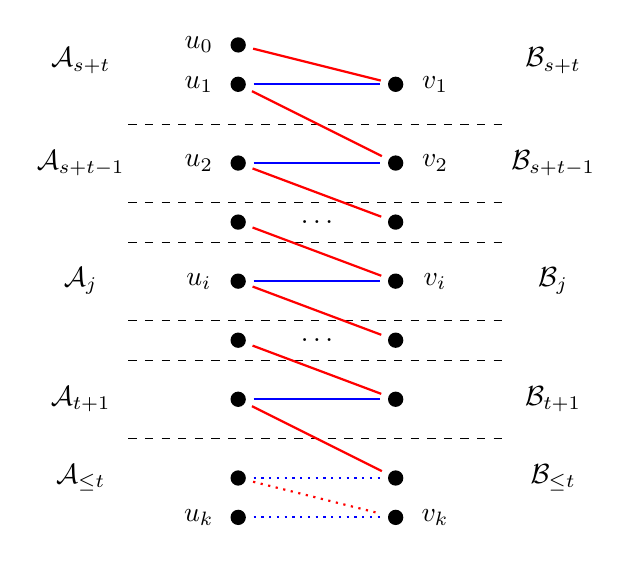
\begin{tikzpicture}[thick,
  lnode/.style={draw=white,fill=blue},
  fsnode/.style={draw,circle,fill=black,scale=0.5},
  every fit/.style={ellipse,draw,inner sep=-2pt,text width=0.5cm},
  -,shorten >= 3pt,shorten <= 3pt
]

% % the vertices of A U B
% \node at (0,1) {$\AA'$};
% \node at (2,1) {$\BB'$};

  \node[fsnode] (u0) at (0,0.5) {};
  \node at (-0.5,0.5) {$u_0$};
  \node[fsnode] (v1) at (2,0) {};
  \node at (2.5,0) {$v_1$};
  \node[fsnode] (u1) at (0,0) {};
  \node at (-0.5,0) {$u_1$};
  \node at (-2,0.3) {$\AA_{\S+\T}$};
  \node at (4,0.3) {$\BB_{\S+\T}$};
   \draw[ultra thin, dashed](-1.5,-0.5) -- (3.5,-0.5);
   
  \node[fsnode] (v2) at (2,-1) {};
  \node at (2.5,-1) {$v_2$};
  \node[fsnode] (u2) at (0,-1) {};
  \node at (-0.5,-1) {$u_2$};
   \node at (-2,-1) {$\AA_{\S+\T-1}$};
   \node at (4,-1) {$\BB_{\S+\T-1}$};
   \draw[ultra thin,dashed](-1.5,-1.5) -- (3.5,-1.5);
   
   \node[fsnode] (ui1) at (0,-1.75) {};
   \node[fsnode] (vi1) at (2,-1.75) {};
   \node at (1,-1.75) {$\ldots$};
   \draw[ultra thin,dashed](-1.5,-2) -- (3.5,-2);
   
  \node[fsnode] (vi) at (2,-2.5) {};
  \node at (2.5,-2.5) {$v_i$};
  \node[fsnode] (ui) at (0,-2.5) {};
  \node at (-0.5,-2.5) {$u_i$};
   \node at (-2,-2.5) {$\AA_{j}$};
  \node at (4,-2.5) {$\BB_{j}$};
   \draw[ultra thin, dashed](-1.5,-3) -- (3.5,-3);
   
   \node[fsnode] (ui11) at (0,-3.25) {};
   \node[fsnode] (vi11) at (2,-3.25) {};
   \node at (1,-3.25) {$\ldots$};
   \draw[ultra thin, dashed](-1.5,-3.5) -- (3.5,-3.5);

\node[fsnode] (vk1) at (2,-4) {};
 % \node at (2.7,-4) {$v_{k-1}$};
  \node[fsnode] (uk1) at (0,-4) {};
  %\node at (-0.6,-4) {$u_{k-1}$};
   \node at (-2,-4) {$\AA_{\T+1}$};
  \node at (4,-4) {$\BB_{\T+1}$};
   \draw[ultra thin, dashed](-1.5,-4.5) -- (3.5,-4.5);
   
   \node[fsnode] (vk) at (2,-5) {};
  %\node at (2.5,-5) {$v_{k}$};
  \node[fsnode] (uk) at (0,-5) {};
  %\node at (-0.5,-5) {$u_{k}$};
   \node at (-2,-5) {$\AA_{\le \T}$};
  \node at (4,-5) {$\BB_{\le \T}$};
  % \draw[ultra thin, dashed](-1.5,-5.5) -- (3.5,-5.5);
  
   % \node[fsnode] (vk11) at (2,-6) {};
  % \node at (2.7,-6) {$v_{k+1}$};
  %  \node at (-2,-6) {$\AA_{\T}$};
  % \node at (4,-6) {$\BB_{\T}$};
  \node[fsnode] (vk11) at (2,-5.5) {};
  \node at (2.5,-5.5) {$v_{k}$};
  \node[fsnode] (uk11) at (0,-5.5) {};
  \node at (-0.5,-5.5) {$u_{k}$};

% % the M edges
 \draw[thick, red ](u0) -- (v1);
 \draw[thick, blue](u1) -- (v1);
 \draw[thick, red ](u1) -- (v2);
 \draw[thick, blue](u2) -- (v2);
 \draw[thick, blue](ui) -- (vi);
 \draw[thick, red ](u2) -- (vi1);
 \draw[thick, red ](ui1) -- (vi);
 \draw[thick, red ](ui) -- (vi11);
 \draw[thick, red ](ui11) -- (vk1);
 \draw[thick, blue](uk1) -- (vk1);
 \draw[thick, red ](uk1) -- (vk);
 \draw[thick, dotted,blue](uk) -- (vk);
 \draw[thick, dotted, red ](uk) -- (vk11);
 \draw[thick, dotted,blue](uk11) -- (vk11);

%  \draw[dashed](g0) -- (h1);
%  \draw[dashed](g1) -- (h2);
%  \draw[dashed](gi) -- (hi1);
% \draw[dashed](g1') -- (h0);
% \draw[dashed](g2') -- (h1');
% \draw[dashed](gi1') -- (hi');
\end{tikzpicture}}
\end{center}

\caption{Blue colored edges denote the edges in $M^*$ whereas red edges denote the edges in $N^*$. }
\label{fig:critLem}
\end{figure}

%\noindent\textbf{The path $\rho$ must contain a clone in $\AA_{x}$ for $x\le \T$:}  
%By the construction of the graph $G_M$, all the clones in $\AA_x$ for $x>\T$ are critical clones for some \emph{lq}-vertex. Thus, if $\rho$ does not contain any vertex $u_i$ such that $u_i\in \AA_{x}$ for $x\le\T$, then all the vertices of $\rho\cap \AA'$ are critical clones, and hence $N^*$ cannot match more critical clones than the matching $M^*$ from $\rho\cap\AA'$. This implies that $\rho$ must contain a clone in $\AA_{x}$ for $x\le\T$. Now, we show that the path $\rho$ must contain at least one clone from each partition class $\AA_{x}$ for $x\ge \T+1$.  Now, we show that the path $\rho$ must contain at least one clone from each partition class $\AA_{x}$ for $x\ge \T+1$. 

By Lemma~\ref{lem:noSteepMM}, we know that $G_M$ does not contain steep downward edges. 
%Hence, we conclude that $v_2\in \BB_x$ and $M^*(v_2)=$ $u_2\in\AA_x$ for $x\in\{\S+\T,\S+\T-1\}$. 
Hence, if $u_i\in\AA_x$ and $u_{i+1}\in\AA_y$ then $x-y\le 1$ for all indices $i$ on $\rho$ and hence, $\rho$ must contain at least one clone from each $\AA_x$ for $\T+1\le x\le \S+\T$ (see Figure~\ref{fig:critLem}). %Let us assume that $u_k\in\AA_{\T}$. Thus, $u_{k-1}\in \AA_y$ for $y\le \T+1$. 
%We remark that the last vertex $u_k$ and the starting vertex $u_0$ of $\rho$, both cannot be the clones of the vertex $a$; otherwise, we get a contradiction that $N^*$ matches more critical clones in $\rho\cap\AA'$ than the matching $M^*$.
%\textcolor{red}{we need to address whether path ends in A or B} \clrP{(Keshav: I believe that the above argument is independent of whether the path ends in $\AA'$ or in $\BB'$. However, we may need to refine the definition of $\rho$. In its current form, $\rho$ always ends on the $\AA'$-side. Should we instead define $\rho$ as follows? `` Let $\rho=\langle u_0, v_1,u_1,v_2,u_2,\ldots,v_k,u_k,\ldots, w_p\rangle$, where $(v_i,u_i)\in M^*$ and the other edges of $\rho$ are in the matching $N^*$. Here, $u_0$ is a critical clone of some vertex $a\in\AA$ which is unmatched in $M^*$, \textbf{and the last clone $w_p$ can be in either $\AA'$ or $\BB'$}.'' I believe that the above arguments remain valid even after this change in the definition of $\rho$. The only thing we need to show that if $w_p\in \AA'$ then $w_p\in \bigcup_{x\le \T} \AA_x$, and if $w_p\in \BB'$ then the penultimate clone on $\rho$ is in $\bigcup_{x\le \T} \AA_x$. Therefore, $\rho$ contains a clone in $\bigcup_{x\le \T} \AA_x$.)}
Now notice that there are at least two clones $u_0$ and $u_1$ in $\AA_{\S+\T}$ and at least one clone in each $\AA_x$ for $\T+1\le x\le \S+\T-1$. As all clones in $\bigcup_{x=\T+1}^{\S+\T}\AA_x$ are critical, there are at least $\S+1$ many critical clones in $\rho\cap \AA'$ contradicting the fact that there are  $s$ critical clones in $\AA'$.

The other case is when $\rho$ ends in $\BB'$, say at $v_{k+1}$. Then $v_{k+1}$ must be unmatched in $M^*$, and hence must be in $\BB_0$ or $\BB_{\T}$ by level-wise partitioning of clones. %Since $v_{k+1}$ is unmatched in $M^*$, 
Also, by Property~\ref{property:GM}(~\ref{obs:partitionPorp6}) and Property~\ref{property:GM}(~\ref{obs:partitionPorp5}), all neighbors of $v_{k+1}$, and hence $u_k$ in particular, must be in $\AA_0$ or $\AA_t$ respectively. Now the same argument as above holds. 
%
% \noindent\textbf{The path $\rho$ ends at some clone $v_{k}\in\BB'$:} This implies that $v_{k}$ is unmatched in $M^*$ and hence $v_{k}\in \BB_y$ for $y\le \T$. 
% %Applying Lemma~\ref{lem:noSteepMM} we see that $u_{k-1}\in\AA_x$ for $x\le \T+1$. 
% Now, repeating the same argument as in the previous case we find that there are at least $\S+1$ many clones in $\bigcup_{x=\T+1}^{\S+\T}\AA_x$ in $G_M$. Thus, we get a contradiction.
%This completes the proof that $M$ is critical for vertices in $\AA$. 

 \vspace{0.1in}

\noindent \textbf{Proof of ($\BB$-part):}
Proof of this part is similar to that of $\AA$-part. For the sake of contradiction, let us assume that $\Dfb{N}<\Dfb{M}$. This implies that there exists an alternating path $\rho$ in $M^*\oplus N^*$ such that $N^*$ matches more critical clones in $\rho\cap\BB'$ than the matching $M^*$. It can be shown that the number of critical clones in $\rho \cap \BB'$ is more than the number of critical clones in $\BB'$, which is a contradiction. 

 The path $\rho$ must start at a clone in $\BB_0$ must end at a clone in $\BB_x $ where $x \ge t$ or at a clone in $\AA_t \cup \AA_{s+t}$. As above, in either case, the path has at least one critical clone in each of  $\BB_1, \ldots, \BB_{t-1}$ and at least two clones in $\BB_0$ accounting for a total of $t+1$ critical clones in $\rho \cap \BB'$, a contradiction to the number of critical clones in $\BB'$.
\end{proof}



\begin{lemma}\label{lem:rwsmMM}
The output matching $M$ is \RSM\ for $G$.
\end{lemma}

\begin{proof}
    If there is no blocking pair w.r.t. $M$, there is nothing to prove. So, let us assume that a blocking pair $(a,b)$ w.r.t. $M$ exists in $G$. By Claim~\ref{cl:blockingUpwards}, there exists $k,r$ such that $(a_k,b_r)$ is a blocking pair w.r.t. $M^*$ in $G_M$. Let us consider the blocking pair $(a_i,b_j)$ w.r.t. $M^*$ such that $a_i$ is in the lowest level ($a_i\in\AA_x$ for the lowest value of $x$), and $b_j$ is in the highest level ($b_j\in \BB_y$ for the highest value of $y$) among all such blocking pairs. We justify the blocking pair $(a,b)$ w.r.t. $M$ in $G$ using edge $(a_i,b_j)$ in $G_M$. That is, we show that the blocking pair $(a,b)$ w.r.t. $M$ is justified either from $a$-side using $a_i$ or from the $b$-side using $b_j$.

    Let $b_j\in\BB_y$. We consider three different cases: $y\le \T-1$,  $y=\T$, and $y>\T$.

    \begin{enumerate}[left=10pt, label = Case \arabic*.]
        \item \textbf{$y\le \T-1$:} By Claim~\ref{cl:blockingUpwards}, $a_i\in\AA_x$ for $x<\T-1$. By Claim~\ref{cl:twoConscutiveL}, all the clones of $a$ are in $\AA_z$ for $z\le \T-1$. Since $a$ did not achieve the level $\T$, we conclude that $a$ is fully subscribed in $M$. This further implies that each $b'\in M(a)$ contains a vertex at a level below $\T$, and hence the capacity of $b'$ is set to $q^-(b')$. Thus, no matched partner of $a$ is surplus in $M$. Hence, the blocking pair $(a,b)$ w.r.t. $M$ is justified from $a$-side.


        \item \textbf{$y=\T$:} By Claim~\ref{cl:blockingUpwards}, $a_i\in\AA_x$ for $x \le \T-1$. This implies $a$ did not exhaust its preference list at level $\T$; hence, $a$ is fully subscribed. Our goal is to show that for any $b'\in M(a)$ such that $b\succ_a b'$, it must be the case that $|M(b')|\le q^-(b')$. Note that if $b'\in M(a)$ such that a clone $b'_k$ of $b'$ is in $\BB_z$ for $z<\T$, then, by the design of our algorithm, $|M(b')|\le q^-(b')$. Thus, when $b'$ is matched to some $a'$ at a level below $\T$, it is not surplus. %; hence, it does not matter whether $b'\succeq_a b$ or $b'\prec_a b$. 
        Therefore, we focus on each $b'\in M(a)$ who does not have any of its matched partners below $\T$. So, let $b'\in M(a)$ be such that all the clones of $b'$ are in $\BB_z$ for $z\ge \T$. We show that $b'\succeq_a b$ and hence it does not matter whether $b'$ is surplus or not.% $|M(b')|>q^-(b')$ or not.

        Note that all the clones of $a$ are in two consecutive levels. As argued above, if a clone of $a$ is in $\AA_x$ for $x<\T$, then the corresponding matched partner cannot be surplus. So, consider the clones of $a$ in $\AA_{\T}$. Let $a_w$ be an arbitrary clone of $a$ such that $a_w\in \AA_{\T}$. Since $a$ is fully subscribed, $a_w$ is matched in $M^*$. Let $M^*(a_w)=b'_p$ be a clone of $b'$. Now, we show that $b'\succeq_a b$.

        Suppose for contradiction $b\succ_a b'$. The fact that  $M^*(a_w)=b'_p$ implies that $a^{\T}$ proposed to $b'$. This further implies that $a^{\T}$ proposed to $b$. Since $(a,b)\notin M$, we conclude that no clone of $b$ is in $\BB_y$ for $y<\T$. This also implies that $b$ is fully subscribed; otherwise, it would not have rejected $a^\T$. Moreover, since $(a,b)$ is a blocking pair, there must exist some $a'\in M(b)$ such that $a\succ_b a'$. Clearly, $a'$ is at level $z>\T$, otherwise, $b$ could not have rejected $a^{\T}$. Therefore, there exists a clone $b_k$ of $b$ such that $b_k\in \BB_z$ for $z>\T$. This contradicts the choice of the clone $b_j$. 

        \item \textbf{$y>\T$:} We consider two different cases -- $a_i\in \AA_x$ for $x< \T$ and $a_i\in \AA_x$ for $x\ge \T$.
        
        \begin{enumerate}[left=-10pt, label = Case (\roman*)]
        \item $a_i\in \AA_x$ for $x< \T$: Clearly, $a$ is fully subscribed in $M$ and $a^\T$ did not exhaust its preference list. If all the clones of $a$ are in $\AA_x$ for $x<\T$, then the blocking pair $(a,b)$ is justified from $a$-side, and we are done (as discussed in the previous cases). Thus, let us assume that there exists a clone $a_p$ of $a$ such that $a_p\in \AA_{\T}$. By Claim~\ref{cl:twoConscutiveL}, $a_i\in \AA_{\T-1}$. If all $b'\in M(a)$ such that $b\succ_a b'$ have at least one clone in $\BB_y$ for $y<\T$, then we are done as the blocking pair is justified from $a$-side ($a$ is fully-subscribed and no lower preferred matched partner of $a$ is surplus). So, let us assume that there exists $b''\in M(a)$ such that $b\succ_a b''$ and all the clones of $b''$ are in $\BB_y$ for $y\ge \T$. This implies $a^\T$ proposed to $b''$, and hence $a^\T$ also proposed to $b$. Since $(a,b)\notin M$, we conclude that no clone of $b$ is in $\BB_y$ for $y<\T$. This also implies that $b$ is fully subscribed; otherwise, it would not have rejected $a^\T$. %Note that the capacity of $b$ is equal to $q^+(b)$ as no matched partner is at a level below $\T$. 
        Since $a^\T$ proposed to $b$ and $b$ rejected it, it must be the case that each $a'\in M(b)$ such that $a\succ_b a'$ is at level $x>\T$. By the design of our algorithm, the capacity of $a'$ is equal to $q^-(a')$. Thus, no lower preferred matched partner of $b$ than $a$ is surplus. This concludes that the blocking pair $(a,b)$ is justified from $b$-side.  

        \item $a_i\in \AA_x$ for $x\ge \T$: Clearly, $a^\T$ proposed to $b$ and $b$ rejected it. Thus, no clone of $b$ is in $\BB_y$ for $y<\T$. This also implies that $b$ is fully subscribed. Since $(a,b)$ is a blocking pair, no lower-preferred matched partner of $b$ can be at a level below $\T+1$. Therefore, no $a'\in M(b)$ such that $a\succ_b a'$ is surplus. Hence the blocking pair $(a,b)$ is justified from $b$-side. 
        
        \end{enumerate}
    \end{enumerate}
    Thus, in all three cases, the blocking pair $(a,b)$ is justified either from $a$-side or from the $b$-side. Hence, $M$ is an $\RSM$.
\end{proof}




\begin{remark}
   Gergely Cs{\'a}ji, in his work ~\cite{csaji2024AAMAS}, introduced a stronger definition of critical relaxed stability by strengthening it in a natural way: for the one-to-one setting, a matching $M$ is critical relaxed stable if it is critical and has no blocking pair $e=(a,b)$ such that replacing $(a, M(a))$ and $(b, M(b))$ with $e$ in $M$ preserves criticality.   He proved that a critical relaxed stable matching always exists under this stronger definition. Using Lemma~\ref{lem:equivCsaji} below, we show that the output of our algorithm satisfies the strengthened definition of criticality.
\end{remark}

\begin{lemma}\label{lem:equivCsaji}
     Let $M$ be the output of Algorithm~\ref{algo:maxCRSMM}. Then there does not exist an edge  $(a,b) \in E \setminus M$ such that for some $a'\in M(b)$ with $a\succ_b a'$ and for some $b'\in M(a)$ with $b \succ_a b'$, and the matching $N = M \setminus \{(a, b'), (a', b)\} \cup \{(a, b)\} $ is also critical. 
     
     
\end{lemma}

\begin{proof}
    We remark that the edge $(a, b)$ by the conditions of the lemma is a blocking pair with respect to $M$. Suppose for contradiction, there exists such blocking pair $(a,b)$. 
    %Since the matching $N =  M \setminus \{(a, b'), (a', b)\} \cup \{(a, b)\} $ is critical, t
    The following three cases are possible. 
   \begin{enumerate}[left=10pt, label = Case \arabic*.]
        \item \label{itm:case1} \textbf{Both $a'$ as well as $b'$ are surplus in the matching $M$.} Clearly, the blocking pair $(a,b)$ is not justified by either of its end-points; a contradiction to the fact that $M$ is a \RSM.
        \item \label{itm:case2} \textbf{$b'$ is not surplus in $M$.} In this case, $N =  M \setminus \{(a, b'), (a', b)\} \cup \{(a, b)\} $ leaves a critical position of the vertex $b'$ unmatched. Since $N$ is a critical matching, it must fill a critical position for some other vertex on $\BB$-side. This can happen only if $b$ is deficient in $M$ and $|N(b)|> |M(b)|$. This implies  $a'=\bot$.   Since $b \succ_a b'$, the vertex $a$ must have proposed $b$ before proposing $b'$. The fact that $(a,b)\notin M$ implies that $b$ rejected $a$ which cannot happen if $b$ is deficient in $M$. 
        \item \label{itm:case3} \textbf{$a'$ is not surplus in $M$.} As in the previous case, $a$ is deficient in $M$ and $b' = \bot$. This implies $a$ proposed $b$ at the highest level $\S+\T$. Since $(a,b)\notin M$, the vertex $b$ rejected $a$. This implies that for each $a''\in M(b)$, we have that $a''\succ_b a$;  a contradiction to the fact that $a\succ_b a'$.
        %\item \label{itm:case4} \textbf{neither of $a'$ and $b'$ is surplus in $M$.} As in previous cases, it must be the case that both $a$ as well as $b$ are deficient in $M$. Now, the proof is the same as the one in \ref{itm:case2} or \ref{itm:case3} above.
    \end{enumerate}  
    Therefore, we conclude that there is no blocking pair with the assumed property. 
\end{proof}

\begin{lemma}\label{lem:2by3RSMmm}
Let $M$ be the output of Algorithm~\ref{algo:maxCRSMM} and $M_{max}$ be any maximum size \CRSM\ for an instance of our problem. Then $|M|\ge \frac{2}{3}|M_{max}|$.
\end{lemma}
  \begin{proof}
 We show that the symmetric difference of $M$ and $M_{max}$ does not admit a 1-length augmenting path\footnote{A 1-length augmenting path w.r.t. $M$ is an edge $(a,b)\notin M$ such that both $a$ and $b$ are under-subscribed in $M$.} or a 3-length augmenting path\footnote{A 3-length augmenting path w.r.t. $M$ is a 3-length path $\langle a',b,a,b'\rangle$ such that $(a,b)\in M$, $(a',b), (a,b')\notin M$ and both $a'$ and $b'$ are under-subscribed in $M$.} w.r.t. $M$. This immediately implies that $|M_{max}|\le \frac{3}{2}\cdot |M|$. Since $M$ is $\RSM$, it is a maximal matching, and hence the symmetric difference of $M$ and $M_{max}$ does not admit 1-length augmenting path w.r.t. $M$.

 Given $M_{max}$, we can construct a level-based cloned graph $G_M$ as done in the proof of Lemma~\ref{lem:CriticalM}. Let us assume that $M^*$ and $M_{max}^*$ are the corresponding one-to-one matchings in $G_M$ for many-to-many matchings $M$ and $M_{max}$, respectively. Let us consider the subgraph $M^*\oplus M_{max}^*$. For the sake of contradiction let us assume that $M^*\oplus M_{max}^*$ contains a 3-length augmenting path $\rho=\langle \Tilde{a}_1,b_1,a_1,\Tilde{b}_1\rangle$ with respect to $M^*$ such that $(a_1,b_1)\in M^*$ and the other two edges are in $M_{max}^*$. Also, assume that $\Tilde{a}_1, b_1, a_1, \Tilde{b}_1$ are clones of $\Tilde{a}, b, a, \Tilde{b}$ respectively. 

 \vspace{0.05in}
 
 \noindent\textbf{Levels of clones $a_1$ and $\Tilde{a}_1$:} Note that $\Tilde{a}$ is under-subscribed in the matching $M$, which implies that $\Tilde{a}^{t^*}$ exhausted its preference list. This further implies that $b_1\in \BB_{y}$ for $y\ge \T$. If $|M(b)|<q^+(b)$ or there exists $a'\in M(b)$ such that $a'$ is at a level below $\T$, then the proposal from $\Tilde{a}^{\T^*}$ must not have been rejected by $b$. Hence, we conclude that $b$ is fully subscribed in $M$ and no $a'\in M(b)$ is at a level below $\T$. This implies $a_1\in \AA_x$ for $x\ge \T$. Note that $\Tilde{b}$ is under-subscribed in $M$. Since $(a,\Tilde{b})\notin M$, $a^{\T}$ did not propose to $\Tilde{b}$ and hence did not exhaust its preference list. Therefore, $a_1\in \AA_{\T}$, which implies that $\Tilde{a}_1\in \AA_{\T}$ (if $\Tilde{a}$ would have achieved a level at least $\T+1$ then $(a,b)\notin M$ -- a contradiction). Hence, $\Tilde{a}_1,a_1\in \AA_\T$.

\vspace{0.05in}

 \noindent\textbf{The pair $(a,b)$ blocks $M_{max}$:}
 The fact that $a$ achieved $\T^{th}$ level, $(a,b)\in M$ and $a^{\T}$ did not propose to $\Tilde{b}$ together imply that $b \succeq_a \Tilde{b}$. This also implies that $a$ did not achieve $\T^*$ status. Suppose $\Tilde{a} \succeq_b a$ then when $\Tilde{a}^{\T^*}$ proposed to $b$, $b$ would have accepted this proposal by rejecting $a$ which is at level at most $\T$. Thus, we conclude that $a\succ_b \Tilde{a}$. Now, we show that $b \succ_a b'$. 
 
 Suppose not. Since $a^\T$ proposed to $b$ before $\Tilde{b}$, it must be the case that $\Tilde{b}\not\succ_a b$. Thus, the only possibility left is that $a$ ranks both $b$ and $\Tilde{b}$ at the same rank, say $k^{th}$-rank, in \prefb. Since $a^{\T}$ did not propose to $\Tilde{b}$, the vertex $\Tilde{b}$ is under-subscribed in $M$ and $(a,b)\in M$; the proposal $(a^{\T},b)$ must be uncertain. We consider two cases: 
\begin{enumerate}[left=0pt, label = Case \arabic*.]
     \item $\Tilde{a}^{\T^*}$ proposed to $b$ before $a^{\T}$ proposed to $b$: Since $\Tilde{b}$ is under-subscribed in $M$, when  $a^{\T}$ proposed to $b$, $b$ must also be under-subscribed in $M$ (if $b$ is fully subscribed, it would not be the favorite neighbor of $a^{\T}$ as $\Tilde{b}$ is under-subscribed).  By the definition of an uncertain proposal, $(\Tilde{a}^{\T^*},b)$ is not an uncertain proposal. We know that $(\Tilde{a},b)\notin M$ and $\Tilde{a}$ is under-subscribed in $M$. This implies that $b$ rejected $\Tilde{a}^{\T^*}$ during the execution of Algorithm~\ref{algo:maxCRSMM}. Since $(a^{\T},b)$ is uncertain proposal, $b$ must reject $a^{\T}$ before rejecting $\Tilde{a}^{\T*}$. Thus, $b$ rejected $a^{\T}$. Since $a^{\T}$ has at least one unproposed and under-subscribed neighbor at the same rank $k$, $a^\T$ cannot propose to $b$ again before proposing to $\Tilde{b}$. The fact that $\Tilde{b}$ is under-subscribed in $M$, and $(a,\Tilde{b})\notin M$ implies that $a^\T$ did not propose to $\Tilde{b}$, and hence did not propose again to $b$. But $(a,b)\in M$ -- a contradiction.
     
     \item $a^{\T}$ proposed to $b$ before $\Tilde{a}^{\T^*}$ proposed to $b$: As discussed earlier, $(a^{\T},b)$ is an uncertain proposal. Note that when $\Tilde{a}^{\T^*}$ proposed to $b$, either $b$ was under-subscribed or fully subscribed in $M$. But in both situations, $b$ receives the proposal from $\Tilde{a}^{\T^*}$. Clearly, $b$ accepts this proposal, possibly by rejecting an uncertain proposal. Since $(\Tilde{a}^{\T^*},b)$ is not an uncertain proposal, $b$ must reject all uncertain proposals before rejecting $\Tilde{a}^{\T^*}$. Thus, $b$ rejected $a^{\T}$ before rejecting $\Tilde{a}^{\T^*}$. Now, $a^\T$ must propose to $\Tilde{b}$ before proposing to $b$ again. The fact that $\Tilde{b}$ is under-subscribed in $M$ and $(a,\Tilde{b})\not\in M$ implies $a^\T$ did not propose to $\Tilde{b}$ and hence again to $b$. But $(a,b)\in M$ -- a contradiction.
 \end{enumerate}
 Therefore, we conclude that $b \succ_a \Tilde{b}$. This establishes that the pair $(a,b)$ blocks $M'$.

 \vspace{0.05in}

\noindent\textbf{The blocking pair $(a,b)$ for $M_{max}$ is not justified:} In order to prove this, we show that $\Tilde{b}$ and $\Tilde{a}$ both are surplus in $M_{max}$. Let us first assume that $\Tilde{b}$ is not surplus in $M_{max}$. Since $|M_{max}(\Tilde{b})|\ge 1$ and $\Tilde{b}$ is not surplus in $M_{max}$, it must be the case that $\Tilde{b}$ is an \emph{lq}-vertex. Thus, $\T=\sum_{b\in \BB}q^-(b)>0$. Recall that no $a'\in M(b)$ is at a level below $\T$, which implies the level of $a$ is at least $\T$. Therefore, $a^0$ exhausted its preference list $\prefslqa$, and hence it must have proposed to $\Tilde{b}$. The vertex $\Tilde{b}$ must have rejected $a^0$, which implies that $\Tilde{b}$ is not deficient in $M$. The non-deficiency of $\Tilde{b}$ in $M$ implies that $\Tilde{b}$ is surplus in $M_{max}$ (if $\Tilde{b}$ is not surplus in $M_{max}$ then $|M_{max}(\Tilde{b})|\le |M(\Tilde{b})|$, and the augmenting path cannot end at $\Tilde{b}_1$ with an $M_{max}^*$ edge). Next, we show that $\Tilde{a}$ is also surplus in $M_{max}$. If $\Tilde{a}$ is not surplus in $M_{max}$ then $q^-(\Tilde{a})>0$, which implies $\S=\sum_{a\in \AA}q^-(a)>0$. Since $\Tilde{a}$ is not surplus in $M_{max}$ we have that $|M_{max}(\Tilde{a})|\le q^-(\Tilde{a})$. Since $\Tilde{a}_1$ is the endpoint of the augmenting path $\rho = \langle \Tilde{a}_1,b_1,a_1,\Tilde{b}_1\rangle$, it must be the case that $|M_{max}(\Tilde{a})|> M(\Tilde{a})$. Thus, $\Tilde{a}$ is deficient in $M$. This implies that $\Tilde{a}^{\S+\T}$ exhausted its preference list {\sf PrefS($\Tilde{a}$)}. Since $\S+\T>\T$, $b$ must accept the proposal from $\Tilde{a}^{\S+\T}$ by possibly rejecting $a^\T$. This implies $(\Tilde{a},b)\in M$ -- a contradiction. 

Thus, $\Tilde{a}$, as well as $\Tilde{b}$, are surplus in $M_{max}$ and hence the blocking pair $(a,b)$ w.r.t. $M_{max}$ is not justified. Therefore, $M_{max}$ is not an $\RSM$.
\end{proof}

Using Lemma~\ref{lem:CriticalM}, Lemma~\ref{lem:rwsmMM} and Lemma~\ref{lem:2by3RSMmm}, we complete the proof of Theorem~\ref{theo:main}.

\section{Conclusion}

In this paper, we study the many-to-many bipartite matching problem with two-sided preferences, where preferences may involve ties and lower quotas are present for agents on both sides of the bipartition. We prove the existence of a critical relaxed stable matching in this setting. Since computing a maximum-size stable matching is NP-hard in instances with ties, even without lower quotas, finding a maximum-size critical relaxed stable matching is also NP-hard.  We present a polynomial-time algorithm that computes a $\frac{3}{2}$-approximation of the maximum-size critical relaxed stable matching. Our approximation factor matches the best-known bound for maximum size (weakly) stable matching in the presence of ties~\cite{mcdermid20093,Kiraly13,paluch2014faster}.



 \bibliographystyle{alphaurl} 
 \bibliography{refs.bib}
\appendix
\newpage
\section{Generalised Kir{\'a}ly's algorithm}\label{append:kiralyMM}
The pseudocode for the adaptation of the Kir{\'a}ly's algorithm~\cite{Kiraly13} to the many-to-many setting is given in Algorithm~\ref{algo:23stableMM}. As mentioned earlier, each vertex $a\in \AA$ proposes to its neighbors until the vertex $a$ is either fully subscribed or has proposed with the $*$ status to all vertices in its preference list. Throughout the algorithm, we use $|M(a)|$ to denote the number of vertices matched to $a$ and $a^*$ combined. During the course of the algorithm, a vertex $a$ can propose $b$ at most three times -- at most two times without $*$ status and at most once with $*$ status. Line~\ref{alg1:upgrade} in Algorithm~\ref{algo:23stableMM} ensures that a vertex $a$ is matched to $b$ at most once. Once a vertex $b\in\BB$ is fully subscribed, it remains fully subscribed throughout the algorithm. Subsequently, for $b$ to receive a proposal from some vertex $a$, the vertex $b$ must be the favorite neighbor of $a$. By the definition of favorite neighbor (Definition~\ref{def:favNbr}), it implies that if $b$ receives a proposal from a vertex $a$, then there does not exist any other neighbor $b'$ at the \emph{same} rank of $b$ for the vertex $a$ such that $b'$ is under-subscribed. Thus, during the course of the algorithm, once a vertex $b$ is fully subscribed, no subsequent proposal to $b$ can be labelled uncertain. We record this as the following observation.


\begin{observation}\label{obs:fullNotuncertain}
Let $b\in\BB$ become fully subscribed at time $t$ during the course of Algorithm~\ref{algo:23stableMM}. Then, after time $t$, no proposal to the vertex $b$ can be labelled as uncertain.
\end{observation}

% During the course of our algorithm, let $M(b)$ for a vertex $b\in \BB$ denote the set of matched partners of $b$ with respect to the current matching $M$. Whenever $b$ receives a proposal from a vertex, say $a$, after $b$ is fully subscribed,  we compare $a$ with some least preferred partners in the set $M(b)$ to decide whether $b$ should accept or reject the proposal by $a$. Therefore, we need to identify the least preferred partners in the set $M(b)$. Note that some vertices in $M(b)$  may have the 
% $*$ status, whereas others may not have the $*$ status.
% %Vertex $b$ prefers a lower-ranked neighbor in $M(b)$ over any higher ranked neighbor in $M(b)$ irrespective of star status of the two vertices. Amongst two vertices having the same rank in $b$'s preference list, 
% %the vertex $b$ prefers a star status neighbor over another neighbor without a star status.  
% Let $j$ be the rank of the highest-ranked neighbor in $M(b)$ for the vertex $b$. If there exists a vertex in $M(b)$ at rank $j$ without $*$ status, then all such vertices are the least preferred partners of $b$. Otherwise (all vertices in $M(b)$ at rank $j$ have star status), all vertices at rank $j$ are the least preferred partners of $b$.

% %Let us assume that vertices $a$ and $\Bar{a}$ are at ranks $i$ and $j$ respectively in $\prefb$. As mentioned earlier, $b$ prefers $a^*$ over a vertex $\Bar{a}$ (vertex $\Bar{a}$ without $*$ status) if and only if $i\le j$. Thus, for any particular rank, say $j$, w.r.t. $\prefb$, we order all the vertices at rank $j$ in $M(b)$ in a way that all $*$  status vertices at rank $j$ are preferred over all vertices at rank $j$ which are without $*$ status. Therefore, the term \textit{lowest preferred} in Algorithm~\ref{algo:23stableMM} refers to the following vertex $\Bar{a}$. Let $a'$ be one of the lowest preferred partners in $M(b)$ and $a'$ is at rank $j$ in $\prefb$. 
% %\begin{itemize}
%  %   \item If there exists $a''\in M(b)$ at rank $j$ in $\prefb$ such that $a''$ is without $*$ status then $\Bar{a}$ refers to any such vertex $a''$.
%   %  \item If all $a'\in M(b)$ at rank $j$ in $\prefb$ are with $*$ status then $\Bar{a}$ refers to any such vertex $a''$.
% %\end{itemize}

\begin{algorithm}
    \caption{$3/2$-approximation of maximum size stable matching in $G = (\AA \cup \BB, E)$ }\label{algo:23stableMM}
    \DontPrintSemicolon
    \SetAlgoLined
    Set $M=\emptyset$, initialize a queue $Q=\{a\ :\ a\in \AA\}$, each $a\in \AA$ unmarks all $b\in \prefa$\;
    
    \While{$Q$ is not empty}{
        let $a=dequeue(Q)$\tcp*{$a$ can be with or without $*$ status}
        \If{$a$ is not with $*$ status}{
            \If{there exists a vertex in $\prefa$ which is marked/unproposed by $a$% has not proposed to all vertices 
            }{
                let $b$ be the favorite neighbor of $a$ at some rank, say $k$\; 
                label uncertain proposals from $a$, if any, at rank $k-1$ as `not uncertain'\;
                \textbf{if} $b$ was marked by $a$ \textbf{then} $a$ unmarks $b$\;
                $a$ proposes to $b$\;
                \If {$b$ is under-subscribed}{
                    $M=M\cup \{(a,b)\}$\;
                    \If{ $\exists\ b'\not= b$ at rank $k$ in $\prefa$ with $|M(b')|<q^+(b')$ and $b'$ is unproposed by $a$}{
                    label $(a,b)$ as an uncertain proposal\tcp*{the first proposal by $a$ to $b$}}
                    }
                \Else{ %b is fully subscribed
                    \If {$\exists \ a'\in M(b)$ such that $(a',b)$ is uncertain}{
                        % Let $a''$ be one of such $a'\in M(b)$\; 
                        $M=(M\setminus \{(a',b)\}) \cup \{(a,b)\}$\;
                        $a'$ marks $b$ \label{alg1:mark}\;
                        add $a'$ to $Q$ if $a'\notin Q$
                    }
                    \Else{%no proposal to $b$ is uncertain and b is fully subscribed
                        let $a'$ be one of the \textit{least preferred} partners in $M(b)$\;
                        \If {$a\succ_b a'$}
                        {
                            $M=(M\setminus \{(a',b)\}) \cup \{(a,b)\}$\;
                            add $a'$ to $Q$ if $a'\notin Q$
                        }
                    }
                }
                \textbf{if} $|M(a)|< q^+(a)$ and $a\notin Q$ \textbf{then} add $a$ to $Q$\label{alg1:underSubA11}\;
        }
        \textbf{else}  add $a^*$ to $Q$ if $a\notin Q$ \tcp*{$a^*$ proposes from the begining of $\prefa$}
        }
        \Else
        {
            \If{$a^*$ has not proposed to all vertices in $\prefa$}{
            let $b$ be the favorite neighbor of $a^*$\;
            \If{$a\in M(b)$}{$M=(M\setminus\{(a,b)\})\cup \{(a^*,b)\}$ \label{alg1:upgrade}\;}
            \Else{
                $a^*$ proposes to $b$ \tcp*{$b$ is full \& no proposal to $b$ is labelled uncertain}
                % no proposal to b can be uncertain at this moment
                let $a'$ be one of the \textit{least preferred} partners in $M(b)$ \;
                \If{$a =_b a'$ and $a'$ is without $*$ status } 
                {
                    $M=(M\setminus \{(a',b)\}) \cup \{(a^*,b)\}$ and add $a'$ to $Q$ if $a'\notin Q$\;
                }
            }
            \textbf{if} $|M(a)|< q^+(a)$ and $a\notin Q$ \textbf{then} add $a^*$ to $Q$ \label{alg1:underSubA12}\;}
        }
}
return $M$\;
\end{algorithm}




% \begin{algorithm}
%     \caption{$3/2$-approximation stable matching in $G = (\AA \cup \BB, E)$ }\label{algo:23stableMM}
%     \DontPrintSemicolon
%     \SetAlgoLined
%     Set $M=\emptyset$, initialize a queue $Q=\{a\ :\ a\in \AA\}$\;
    
%     \While{$Q$ is not empty}{
%         Let $a=dequeue(Q)$\tcc*{$a$ can be with or without $*$ status}
%         \If{$a$ is not with $*$ status}{
%             \If{$a$ has not exhausted $\prefa$}{
%                 Let $b$ be the favorite neighbor of $a$ at some rank, say $k$, in $\prefa$\;
               
%                 \If{$\exists \ b'$ at rank $k-1$ in $\prefa$ such that $(a,b')$ is an uncertain proposal}{Label all such uncertain proposals involving $a$ as `not uncertain'}
                
%                 \textbf{if} $b$ was marked by $a$ \textbf{then} $a$ unmarks $b$\;
%                 $a$ proposes to $b$\;
%                 \If {$b$ is under-subscribed}{
%                     $M=M\cup \{(a,b)\}$\;
%                     \If{ $\exists\ b'\not= b$ at rank $k$ in $\prefa$ with $|M(b')|<q^+(b')$ and $b'$ is unproposed by $a$}{
%                     Label $(a,b)$ as an uncertain proposal\tcc*{the first proposal by $a$ to $b$}}
%                     }
%                 \Else{ %b is fully subscribed
%                     \If {$\exists \ a'\in M(b)$ such that $(a',b)$ is uncertain}{
%                         Let $a''$ be one of such $a'\in M(b)$\; 
%                         $M=(M\setminus \{(a'',b)\}) \cup \{(a,b)\}$\;
%                         $a''$ marks $b$ \label{alg1:mark}\;
%                         add $a''$ to $Q$ if $a''\notin Q$
%                     }
%                     \Else{%no proposal to $b$ is uncertain and b is fully subscribed
%                         Let $a'$ be one of the lowest preferred partners in $M(b)$ and $a'$ is at rank $j$ in $\prefb$\;
%                         \If {$\exists \ a''\in M(b)$ at rank $j$ in $\prefb$ such that $a''$ is without $*$ status }{
%                             Let $\Bar{a}$ be one of such $a''$\;
%                         }
%                         \uElseIf {all $a''\in M(b)$ at rank $j$ in $\prefb$ are with $*$ status }{
%                             Let $\Bar{a}$ be one of such $a''$\;
%                         }
%                         \If {$a\succ_b \Bar{a}$}
%                         {
%                             $M=(M\setminus \{(\Bar{a},b)\}) \cup \{(a,b)\}$\;
%                             add $\Bar{a}$ to $Q$ if $\Bar{a}\notin Q$
%                         }
%                     }
%                 }
%                 \textbf{if} $|M(a)|< q^+(a)$ and $a\notin Q$ \textbf{then} add $a$ to $Q$\label{alg1:underSubA11}\;
%         }
%         \textbf{else if}  $a\notin Q$ \textbf{then} add $a^*$ to $Q$ \tcc*{$a^*$ proposes from the begining of $\prefa$}
%         }
%         \Else
%         {
%             \If{$a^*$ has not exhausted $\prefa$}{
%             Let $b$ be the favorite neighbor of $a^*$\;
%             \If{$a\in M(b)$}{$M=(M\setminus\{(a,b)\})\cup \{(a^*,b)\}$ \;}
%             \Else{
%                 $a^*$ proposes to $b$ \tcc*{$b$ is full \& no proposal to $b$ is labelled uncertain}
%                 % no proposal to b can be uncertain at this moment
%                 Let $a'$ be one of the lowest preferred partners in $M(b)$ and $a'$ is at rank $j$ in $\prefb$\;
%                 \If{$a \succ_b a'$ \textbf{and} $\exists \ a''\in M(b)$ at rank $j$ in $\prefb$ such that $a''$ is without $*$ status }
%                 {
%                     $M=(M\setminus \{(a'',b)\}) \cup \{(a^*,b)\}$ and  add $a''$ to $Q$ if $a''\notin Q$\;
%                 }
%                 \uElseIf{$a \succ_b a'$ \textbf{and} all $a''\in M(b)$ at rank $j$ in $\prefb$ are with $*$ status }
%                 {
%                     $M=(M\setminus \{(a',b)\}) \cup \{(a^*,b)\}$ and add $a'$ to $Q$ if $a''\notin Q$\;
%                 }
%             }
%             \textbf{if} $|M(a)|< q^+(a)$ and $a\notin Q$ \textbf{then} add $a^*$ to $Q$ \label{alg1:underSubA12}\;}
%         }
% }
% Return $M$\;
% \end{algorithm}



\subsection{Correctness of the generalised  Kir{\'a}ly's algorithm}\label{sec:GenKiralyCorr}
To show the correctness, we prove that the matching $M$ output by Algorithm~\ref{algo:23stableMM} is stable and is a $\frac{3}{2}$-approximation to the maximum size stable matching in $G$.




\begin{lemma}\label{lem:stableAlgo2}
The matching $M$ output by Algorithm~\ref{algo:23stableMM} is stable.
\end{lemma}
\begin{proof}
Assume for contradiction that $(a,b)$ is a blocking pair w.r.t. $M$. We consider three cases:
\begin{itemize}
    \item \textbf{$b$ is under-subscribed:} Clearly, $b$ did not receive enough proposals. This implies that $a$ did not propose to $b$. This further implies that $a$ is fully subscribed before proposing to $b$. Hence, $a$ does not strictly prefer $b$ over any matched partners in $M(a)$. This contradicts that $(a,b)$ is a blocking pair.
    
    \item \textbf{$a$ is under-subscribed:} Each time $a$ is under-subscribed, it is added to the queue (see Line~\ref{alg1:underSubA11} and Line~\ref{alg1:underSubA12} of Algorithm~\ref{algo:23stableMM}). It proposes again until it exhausts all the vertices in $\prefa$ with $*$ status or it is fully subscribed. Since $a$ remains under-subscribed, we conclude that $a$ proposed to all vertices in its preference list with the $*$ status. Thus, $a^*$ proposed to $b$ and $b$ rejected $a^*$. This implies that when $a^*$ proposes to $b$, $b$ was fully subscribed with all $a'\in M(b)$ at least as good as $a^*$, and $b$ was not part of any uncertain proposal. This further implies that $a^*$ is not strictly better preferred than any $a'\in M(b)$ at the time when $b$ rejected the proposal from $a^*$. By Observation~\ref{obs:fullNotuncertain}, no proposal to $b$ is labelled uncertain after $b$ is fully subscribed. Since $b$ was not part of any uncertain proposal when it rejected $a^*$, and no proposal to $b$ was labelled uncertain afterwards, $b$ does not accept proposals from lower-preferred vertices than $a$. Thus, $a$ is not strictly better than any $a'\in M(b)$. This contradicts our assumption that $(a,b)$ is a blocking pair.

    \item \textbf{$a$ and $b$ both are fully subscribed:} Since $(a,b)$ is a blocking pair, $a$ must strictly prefer $b$ over some $b'\in M(a)$. This implies $a$ proposed to $b$ before proposing to $b'$. This further implies that $b$ rejected the proposal from $a$. Suppose $b$ rejected $a$ because $b$ is fully subscribed with all the partners as good as $a$ and no partner $a'\in M(b)$ is such that the proposal $(a',b)$ is uncertain. Then, by Observation~\ref{obs:fullNotuncertain}, no proposal to $b$ was labelled uncertain. Since the partners of $b$ do not get worse, $(a,b)$ is not a blocking pair. So, let us assume that $a$ was rejected by $b$ because $(a,b)$ was an uncertain proposal, $b$ was fully subscribed, and $b$ received a proposal from some $a'$.  But, in this case, by the design of the algorithm, $a$ marked $b$ (see Line~\ref{alg1:mark} of Algorithm~\ref{algo:23stableMM}). Since $b'$ is strictly lower preferred than $b$, $a$ must propose to $b$ again before proposing to $b'$ (recall Definition~\ref{def:favNbr}). Also note that when $a$ proposes to $b$ again, the proposal $(a,b)$ is not uncertain as this is not the first proposal to $b$ by $a$. The fact that $b$ rejected $a$  again implies that $b$ was not part of any uncertain proposal when it rejected $a$, and all the partners of $b$ were at least as good as $a$. By Observation~\ref{obs:fullNotuncertain}, no proposal to $b$ was labelled uncertain afterwards; hence, it is not matched to any lower-preferred partner than $a$. Thus, all the partners of $b$ are at least as good as $a$. This is a contradiction that $(a,b)$ is a blocking pair.
\end{itemize}
Thus, the matching $M$ output by Algorithm~\ref{algo:23stableMM} is stable.
\end{proof}

\begin{lemma}\label{lem:23stable}
Let $M$ be the output of Algorithm~\ref{algo:23stableMM} for an instance $G$ and $M_{opt}$ is a maximum size stable matching in $G$ then $|M_{opt}|\le \frac{3}{2}\cdot |M|$.
\end{lemma}

\begin{proof}
    We prove this by showing no 1-length augmenting path\footnote{A 1-length augmenting path w.r.t. $M$ is an edge $(a,b)\notin M$ such that both $a$ and $b$ are under-subscribed in $M$.} or a 3-length augmenting path\footnote{A 3-length augmenting path w.r.t. $M$ is a 3-length path $\langle a',b,a,b'\rangle$ such that $(a,b)\in M$, $(a',b), (a,b')\notin M$ and both $a'$ and $b'$ are under-subscribed in $M$.} exists w.r.t. $M$ in $M_{opt}\oplus M$. Since the matching is stable, it is clear that there does not exist any 1-length augmenting path w.r.t. $M$ in $M_{opt}\oplus M$. Thus, we need to show that there is no 3-length augmenting path w.r.t. $M$ in $M_{opt}\oplus M$. 
    
    Suppose for contradiction that there is a 3-length augmenting path $\langle a_1, b, a, b_1\rangle$ such that $(a,b)\in M$ and the other two edges are in $M_{opt}$.    Clearly, $a_1$ remains under-subscribed in $M$ at the end of the algorithm. This implies that the proposal of $a_1^*$ was rejected by $b$. This further implies that $b$ is fully subscribed, and there is no uncertain proposal involving $b$ when $b$ rejected $a_1^*$. By Observation~\ref{obs:fullNotuncertain}, no proposal to $b$ is labelled uncertain afterwards. Also, note that $b_1$ is under-subscribed in $M$ and $(a,b_1)\notin M$. This implies that $a$ never proposed $b_1$, which further implies that $a$ did not exhaust proposing all vertices in $\prefa$ even without $*$ status. Therefore, $a$ did not achieve the $*$ status during the course of our algorithm. Since $b$ rejected $a_1^*$, we conclude that $a\succ_b a_1$, that is, $b$ ranks $a$ strictly better than $a_1$ in $\prefb$.

    Since $a$ did not propose $b_1$ during the course of Algorithm~\ref{algo:23stableMM}, $a$ is full even before proposing to $b_1$. This further implies that $b_1\not\succ_a b$, that is, $a$ ranks $b$ either strictly better than $b_1$ or at the same rank as $b_1$. Thus, $b \succeq_a b_1$. Now, we show that $b\succ_a b_1$. This immediately contradicts the stability of $M_{opt}$. 
    
    Suppose $b_1=_a b$ such that $b$ and $b_1$ are at $k^{th}$ rank in $\prefa$. Since $a$ is matched to a $k^{th}$-rank neighbor $b$ and an unproposed under-subscribed neighbor $b_1$ exists at the same rank $k$,  the proposal $(a,b)$ is labelled uncertain. Note that $a$ did not propose to any $(k+1)^{th}$-rank neighbor during the course of the algorithm because at least one $k^{th}$-rank neighbor $b_1$ remains unproposed by $a$ at the end of the algorithm. We consider the following two cases based on who among $a_1^*$ and $a$ proposed $b$ first.

\vspace{0.1in}

    \noindent\textbf{$a_1^*$ proposes to $b$ before $a$ proposes to $b$:} As the proposal from $a_1^*$ to $b$ is not the first proposal from $a_1$ to $b$, the proposal $(a_1^*,b)$ cannot be labelled uncertain. Three things can happen when $b$ receives the proposal from $a_1^*$ -- $(i)$ $b$ rejects $a_1^*$, $(ii)$ $b$ accepts $a_1^*$ and is fully subscribed and $(iii)$ $b$ accepts $a_1^*$ and is under-subscribed.  In the first two scenarios, $b$ cannot be the favorite neighbor of $a$ until $b'$ is proposed by $a$. So, $a$ must propose $b_1$ before $a$ proposes $b$. The fact that $(a,b)\in M$, $a$ must have proposed to $b$, which implies $a$ also proposed to $b_1$. Since $b_1$ is under-subscribed, $b_1$ accepts $a$, and hence, $(a,b_1)\in M$ -- a contradiction. In $(iii)$, the proposal, $(a,b)$ is labelled as an uncertain proposal because $b_1$ is under-subscribed and is unproposed by $a$. Since the proposal $(a_1^*,b)$ is not uncertain and $(a,b)$ is uncertain, $b$ must reject $a$ before rejecting $a_1^*$. The fact that $(a_1^*,b)\notin M$ implies that $b$ rejected $a_1^*$ and thus it also rejected $a$. Now, $a$ must propose $b_1$ before proposing to $b$. The fact that $(a,b)\in M$ implies that $a$ proposed to $b$ again, and hence it proposed to $b_1$.  Since $b_1$ is under-subscribed, $b_1$ accepts $a$, and $(a,b_1)\in M$ -- a contradiction.
    

\vspace{0.1in}

     \noindent\textbf{$a$ proposes to $b$ before $a_1^*$ proposes to $b$:} The proposal $(a,b)$ is an uncertain proposal because $b_1$ is under-subscribed and is unproposed by $a$.  The fact that $(a_1,b)\not\in M$ implies $b$ rejected $a_1^*$ ($a_1^*$ must have proposed to $b$ as it remained under-subscribed in $M$). But $(a_1^*,b)$ is not an uncertain proposal. Thus, $b$ must reject $a$ before rejecting $a_1^*$. The fact that $(a_1^*,b)\notin M$ implies that $b$ rejected $a_1^*$ and thus it also rejected $a$. Now, $a$ must propose $b_1$ before proposing to $b$. The fact that $(a,b)\in M$ implies that $a$ proposed to $b$ again, and hence it proposed to $b_1$.  Since $b_1$ is under-subscribed, $b_1$ accepts $a$, and $(a,b_1)\in M$ -- a contradiction.
\end{proof}


%%%%%%%%%%%%%%%%%%%%%%%%%%%%%%%%%%%%%%%%%%%%%%%%%%%%%%%%%%%%%%%%%%%%%%%%%%%%%%%%%%%%%%%%%%%%%%%%%%%%%%%%%%%%%%%%%%%%%%%%%%%%%%%%%%%%%%%%%%%%%%%%%%%%%%%%%%%%%%%%%%%%%%%%%%%%%%%%%%%%

% \begin{algorithm}
%     \caption{$3/2$-approximation stable matching in $G = (\AA \cup \BB, E)$ }\label{algo:23stableMMold}
%     \DontPrintSemicolon
%     \SetAlgoLined
%     Set $M=\emptyset$, initialize a queue $Q=\{a\ :\ a\in \AA\}$\;
    
%     \While{$Q$ is not empty}{
%         let $a=dequeue(Q)$\tcc*{$a$ can be with/without $*$ status}
%             \If{$a$ has not exhausted $\prefa$}{
%                 let $b$ be the favorite neighbor of $a$ in $\prefa$ at some rank, say $k$\;
%                 \textbf{if} $a$ is with $*$ status and $a\in M(b)$ \textbf{then} $M=(M\setminus\{(a,b)\})\cup \{(a^*,b)\}$ and \textbf{continue}\;
%                 % make all such uncertain proposals as `not uncertain'\;
%                 \If{$\exists \ b'$ such that $(a,b')$ is uncertain proposal and $b'$ is $(k-1)^{th}$ rank neighbor in $\prefa$}{make all such uncertain proposals as `not uncertain'}
                
%                 \textbf{if} $b$ was marked by $a$ \textbf{then} $a$ unmarks $b$\;
%                 $a$ proposes to $b$\;
%                 \If {$b$ is under-subscribed}{$M=M\cup \{(a,b)\}$\;
%                 \If{ there exists an under-subscribed $b''$ at rank $k$ which is unproposed by $a$ in $\prefa$ and $a$ never proposed to $b$ earlier with/without $*$ status}{
%                     set $(a,b)$ as uncertain proposal}
%                     }
                
%         % \Else(\tcc*[h]{$b$ is fully subscribed}){
%         \Else{
%             \If {$\exists \ a'\in M(b)$ such that $(a',b)$ is uncertain}{
%                 let $a''$ be the highest indexed agent in $\prefb$ among all such $a'\in M(b)$\; 
%                 $M=(M\setminus \{(a'',b)\}) \cup \{(a,b)\}$\;
%                 $a''$ marks $b$ \label{alg1:marking}\;
%                 add $a''$ to $Q$ if $a''\notin Q$}
%             \uElseIf {%no proposal to $b$ is uncertain and 
%             $\exists\ a'\in M(b)$ such that $a'\prec_b a$}{
%                 let $a''$ be the highest indexed agent amongst lowest preferred partners in $M(b)$\;
%                 $M=(M\setminus \{(a'',b)\}) \cup \{(a,b)\}$\;
%                 add $a''$ to $Q$ if $a''\notin Q$}
%         %         \Else{add $a$ to $Q$ if $a\notin Q$}
%         % % }
%         }
%         \If{$|M(a)|< q^+(a)$ and $a\notin Q$\label{alg1:underSubA21}}{add $a$ to $Q$\label{alg1:underSubA22}\;}}
%         \Else{
%             \If{$a$ is not with $*$ status}{
%                 $a$ achieves $*$ status\;
%                 add $a^*$ to $Q$ \tcc*{$a^*$ proposes from the begining of $\prefa$}}
%         }
% }
% \end{algorithm}



\end{document}

